%%
%% Copyright 2007, 2008, 2009 Elsevier Ltd
%%
%% This file is part of the 'Elsarticle Bundle'.
%% ---------------------------------------------
%%
%% It may be distributed under the conditions of the LaTeX Project Public
%% License, either version 1.2 of this license or (at your option) any
%% later version.  The latest version of this license is in
%%    http://www.latex-project.org/lppl.txt
%% and version 1.2 or later is part of all distributions of LaTeX
%% version 1999/12/01 or later.
%%
%% The list of all files belonging to the 'Elsarticle Bundle' is
%% given in the file `manifest.txt'.
%%

%% Template article for Elsevier's document class `elsarticle'
%% with numbered style bibliographic references
%% SP 2008/03/01

\documentclass[preprint,1p]{elsarticle}
\biboptions{numbers,sort&compress}

%% Use the option review to obtain double line spacing
%% \documentclass[authoryear,preprint,review,12pt]{elsarticle}

%% Use the options 1p,twocolumn; 3p; 3p,twocolumn; 5p; or 5p,twocolumn
%% for a journal layout:
%% \documentclass[final,1p,times]{elsarticle}
%% \documentclass[final,1p,times,twocolumn]{elsarticle}
%% \documentclass[final,3p,times]{elsarticle}
%% \documentclass[final,3p,times,twocolumn]{elsarticle}
%% \documentclass[final,5p,times]{elsarticle}
%% \documentclass[final,5p,times,twocolumn]{elsarticle}

%% For including figures, graphicx.sty has been loaded in
%% elsarticle.cls. If you prefer to use the old commands
%% please give \usepackage{epsfig}

%% The amssymb package provides various useful mathematical symbols
\usepackage{amssymb}
\usepackage{lineno}
\usepackage{hyperref}
\usepackage{siunitx}
\usepackage{multirow}
\usepackage{wasysym}
\usepackage{tabularx}
\usepackage{mathtools}
\usepackage{xcolor}
\usepackage{booktabs,multirow}%
\newcommand{\makecell}[2][@{}c@{}]{\begin{tabular}{#1}#2\end{tabular}}
\usepackage[margin=1in]{geometry}% Just for this example
%\usepackage[percent]{overpic}
%\usepackage[usenames,dvipsnames,svgnames,table]{xcolor}
%\usepackage{cleveref}

%% The amsthm package provides extended theorem environments
%% \usepackage{amsthm}

%% The lineno packages adds line numbers. Start line numbering with
%% \begin{linenumbers}, end it with \end{linenumbers}. Or switch it on
%% for the whole article with \linenumbers.
%% \usepackage{lineno}

\journal{Nucl. Instrum. Meth. A}

\begin{document}

\linenumbers

\begin{frontmatter}

%% Title, authors and addresses

%% use the tnoteref command within \title for footnotes;
%% use the tnotetext command for theassociated footnote;
%% use the fnref command within \author or \address for footnotes;
%% use the fntext command for theassociated footnote;
%% use the corref command within \author for corresponding author footnotes;
%% use the cortext command for theassociated footnote;
%% use the ead command for the email address,
%% and the form \ead[url] for the home page:
%% \title{Title\tnoteref{label1}}
%% \tnotetext[label1]{}
%% \author{Name\corref{cor1}\fnref{label2}}
%% \ead{email address}
%% \ead[url]{home page}
%% \fntext[label2]{}
%% \cortext[cor1]{}
%% \address{Address\fnref{label3}}
%% \fntext[label3]{}

\title{Simulation of the time resolution of a 50~$\mu$m low-gain avalanche detector.}

%% use optional labels to link authors explicitly to addresses:
%% \author[label1,label2]{}
%% \address[label1]{}
%% \address[label2]{}

\author[1,2]{C.~Pe\~na\corref{cor}}\ead{cmorgoth@fnal.gov}
\author[1]{G.~Deptuch}
\author[2]{S.~Xie}
\author[1]{A.~Apresyan}
\author[2]{L.~Narvaez}
\author[1]{T.~Liu}
\author[3]{N.~Cartiglia}


\address[1]{Fermi National Accelerator Laboratory, Batavia, IL, USA}
\address[2]{California Institute of Technology, Pasadena, CA, USA}
\address[3]{INFN, Torino, Italy}
\cortext[cor]{Corresponding author}

\begin{abstract}
%% Text of abstract
In this paper we report simulation results on the timing resolution of a 50~$\mu$m low-gain avalanche detector (LGAD).
The simulation includes: sensor fluctuations, front-end electronics, and time quantization.
Comparisons on the performance for different front-end electonics (FEE) bandwidths (BWs) are presented, as well as
the dependance on singal-to-noise ratio (SNR).
Two approaches to measure the timestamp are considered: leading edge (LE) and constant fraction (CF).
Aditionally, the time resolution is studied as function of the irradiation of the sensor.
Simulated LGAD pulses before irradiation, and after neutron fluences of
 $5\times 10^{14}$~n/cm$^2$ and $1\times 10^{15}$~n/cm$^2$, are studied.
 The time resolution a 50~$\mu$m LGADs was found to be ~35~\si{ps} for FE electronics BWs larger than 350~\si{MHz} and SNRs larger than 30.
 The time resolution at a SNR of 30 for fluences of $5\times 10^{14}$~n/cm$^2$ and $1\times 10^{15}$~n/cm$^2$ were found to be ~31~\si{ps}
  and ~37~\si{ps}, respectively.
\end{abstract}

\begin{keyword}
%% keywords here, in the form: keyword \sep keyword

%% PACS codes here, in the form: \PACS code \sep code
Silicon \sep Timing \sep LGAD
%% MSC codes here, in the form: \MSC code \sep code
%% or \MSC[2008] code \sep code (2000 is the default)

\end{keyword}

\end{frontmatter}

\tableofcontents

%% \linenumbers

%% main text
\section{Introduction}

LGADs are envisioned to be used in the CMS and ATLAS experiment upgrades for HL-LHC in order to overcome
the event reconstruction challenges posed by the high rate of concurrent
collisions per beam crossing (pileup). The implemented regions of pseudorapidity ($\eta$)
are: $1.6< |\eta| <2.9$, and $2.4< |\eta|<4.2$ for CMS and ATLAS, respectively.% In
%order to achieve the desired timing precision across a large area of the
%detectors, the sensors will need to provide high uniformity of signal response
%and timing resolution. Beam test measurements have provided encouraging results towards achieving
%such detectors
 Beam test measurements have demonstrated that the required time resolution,
radiation tolerance, and uniformity of LGAD sensors can be achieved~\cite{Apresyan:2018oln}.
%Si: We need to cite ATLAS testbeam results too right? Do they have it?

In this paper, we report simulation results on the
timing resolution of a 50~$\mu$m LGAD which includes sensor fluctuations,
front-end electronics (FEE) noise, and time quantization.
We scan relevant parameters for timing resolution: analog bandwidths (BWs),
signal-to-noise ratios (SNR), and sensor irradiation.
Our results indicate that for FEE analog BWs larger than 350~\si{MHz},
corresponding to shaping times less than 1~\si{ns}, and SNR larger than 30, time resolutions of 30--37~\si{ps} and 34--47~\si{ps}
are obtained when using constant fraction (CF) and leading edge (LE) discrimintators, respectively.
These results are compatible with previous measurements on LGAD timing resolutions carried out under
laboratory and beam test conditions~\cite{Apresyan:2018oln, Cartiglia201783, PELLEGRINI201412}.
We study the time resolution of four different FEE shaping times: $0.5$~\si{ps}, $1.0$~\si{ps},
$2.0$~\si{ps}, and $4.0$~\si{ps}; three SNR: 20, 30, 100; and three sensor irradiation
levels: pre-radiation, $5\times 10^{14}$~n/cm$^2$, and $1\times 10^{15}$~n/cm$^2$.
For every point in this scan we evaluate the time resolution for LE and CF.
Our results are a guideline on what time resolution can
be achieved for a particular combination of analog bandwidth, SNR, and sensor.

The paper is organized as follows: the simulation is described in
Sec.~\ref{sec:simulation}; algorithms used in the timing
reconstruction and analysis are described in Sec.~\ref{sec:timing_and_analysis}; simulation results
are presented in Sec.~\ref{sec:results}, followed by the conclusion in
Sec.~\ref{sec:conclusion}.

\section{Simulation Framework}
\label{sec:simulation}

%We performed the test-beam measurements at the Fermilab Test-beam
%Facility%

%The simulation framework is based on c++ programing language.  [Si: I don't think we need this right? also there's greg's stuff which is mathematica]
Unprocessed signal pulses from the LGAD sensors are obtained from Weightfield2 (WF2), a 2-dimensional
silicon simulator~\cite{Sadrozinski:2017qpv}. WF2 was used to simulate sets of 1000 signal pulses modeling the
response of minimum-ionizing particles (MIP) traversing the LGAD sensor. Three sets of such signal pulses were
generated for a 50~$\mu$m LGAD sensor at different levels of sensor irradiation: pre-irradiation, and after
neutron fluences of $5\times 10^{14}$~n/cm$^2$ and $1\times 10^{15}$~n/cm$^2$.
Gaussian white noise are added to these unprocessed signals, and the combined waveform is fed into
the simulation of the FEE, illustrated in Fig.~\ref{fig:simulation_diagram} and described in further detail in
Sec.~\ref{sub_sec:fee_simulation_and_noise}. The output of the FEE simulation is the convolution of the
impulse response function and the input signal at the FEE. We consider four shaping constants for the impulse response
of the FEE: 0.5, 1.0, 2.0, and 4.0~\si{ns}. At the output of the FEE block, we obtain simulated processed LGAD pulses,
which include the effects of sensor fluctuations, the shaping of the FEE, and noise. A waveform analysis is performed
with the pulses obtained at the output of the FEE block. We assign timestamps to each pulse by using algorithms that emulate
ideal LE and CF discriminators. For each threshold we obtain an LE and CF timestamp as well as the corresponding
time-over-theshold (ToT) of the pulse. The SNR is defined as the ratio of the most probable value (MPV) of the
amplitude distribution to the width of the amplitude distribution at a fixed sample of noise-only waveforms.
We study three SNR scenarios: 20, 30, and 100. A schematic diagram of the simulation is shown in Fig.~\ref{fig:simulation_diagram}.
 %This simulation implements a more realistic version of a CF discriminator
%based on signal delays.

\begin{figure}[htbp]
\centering
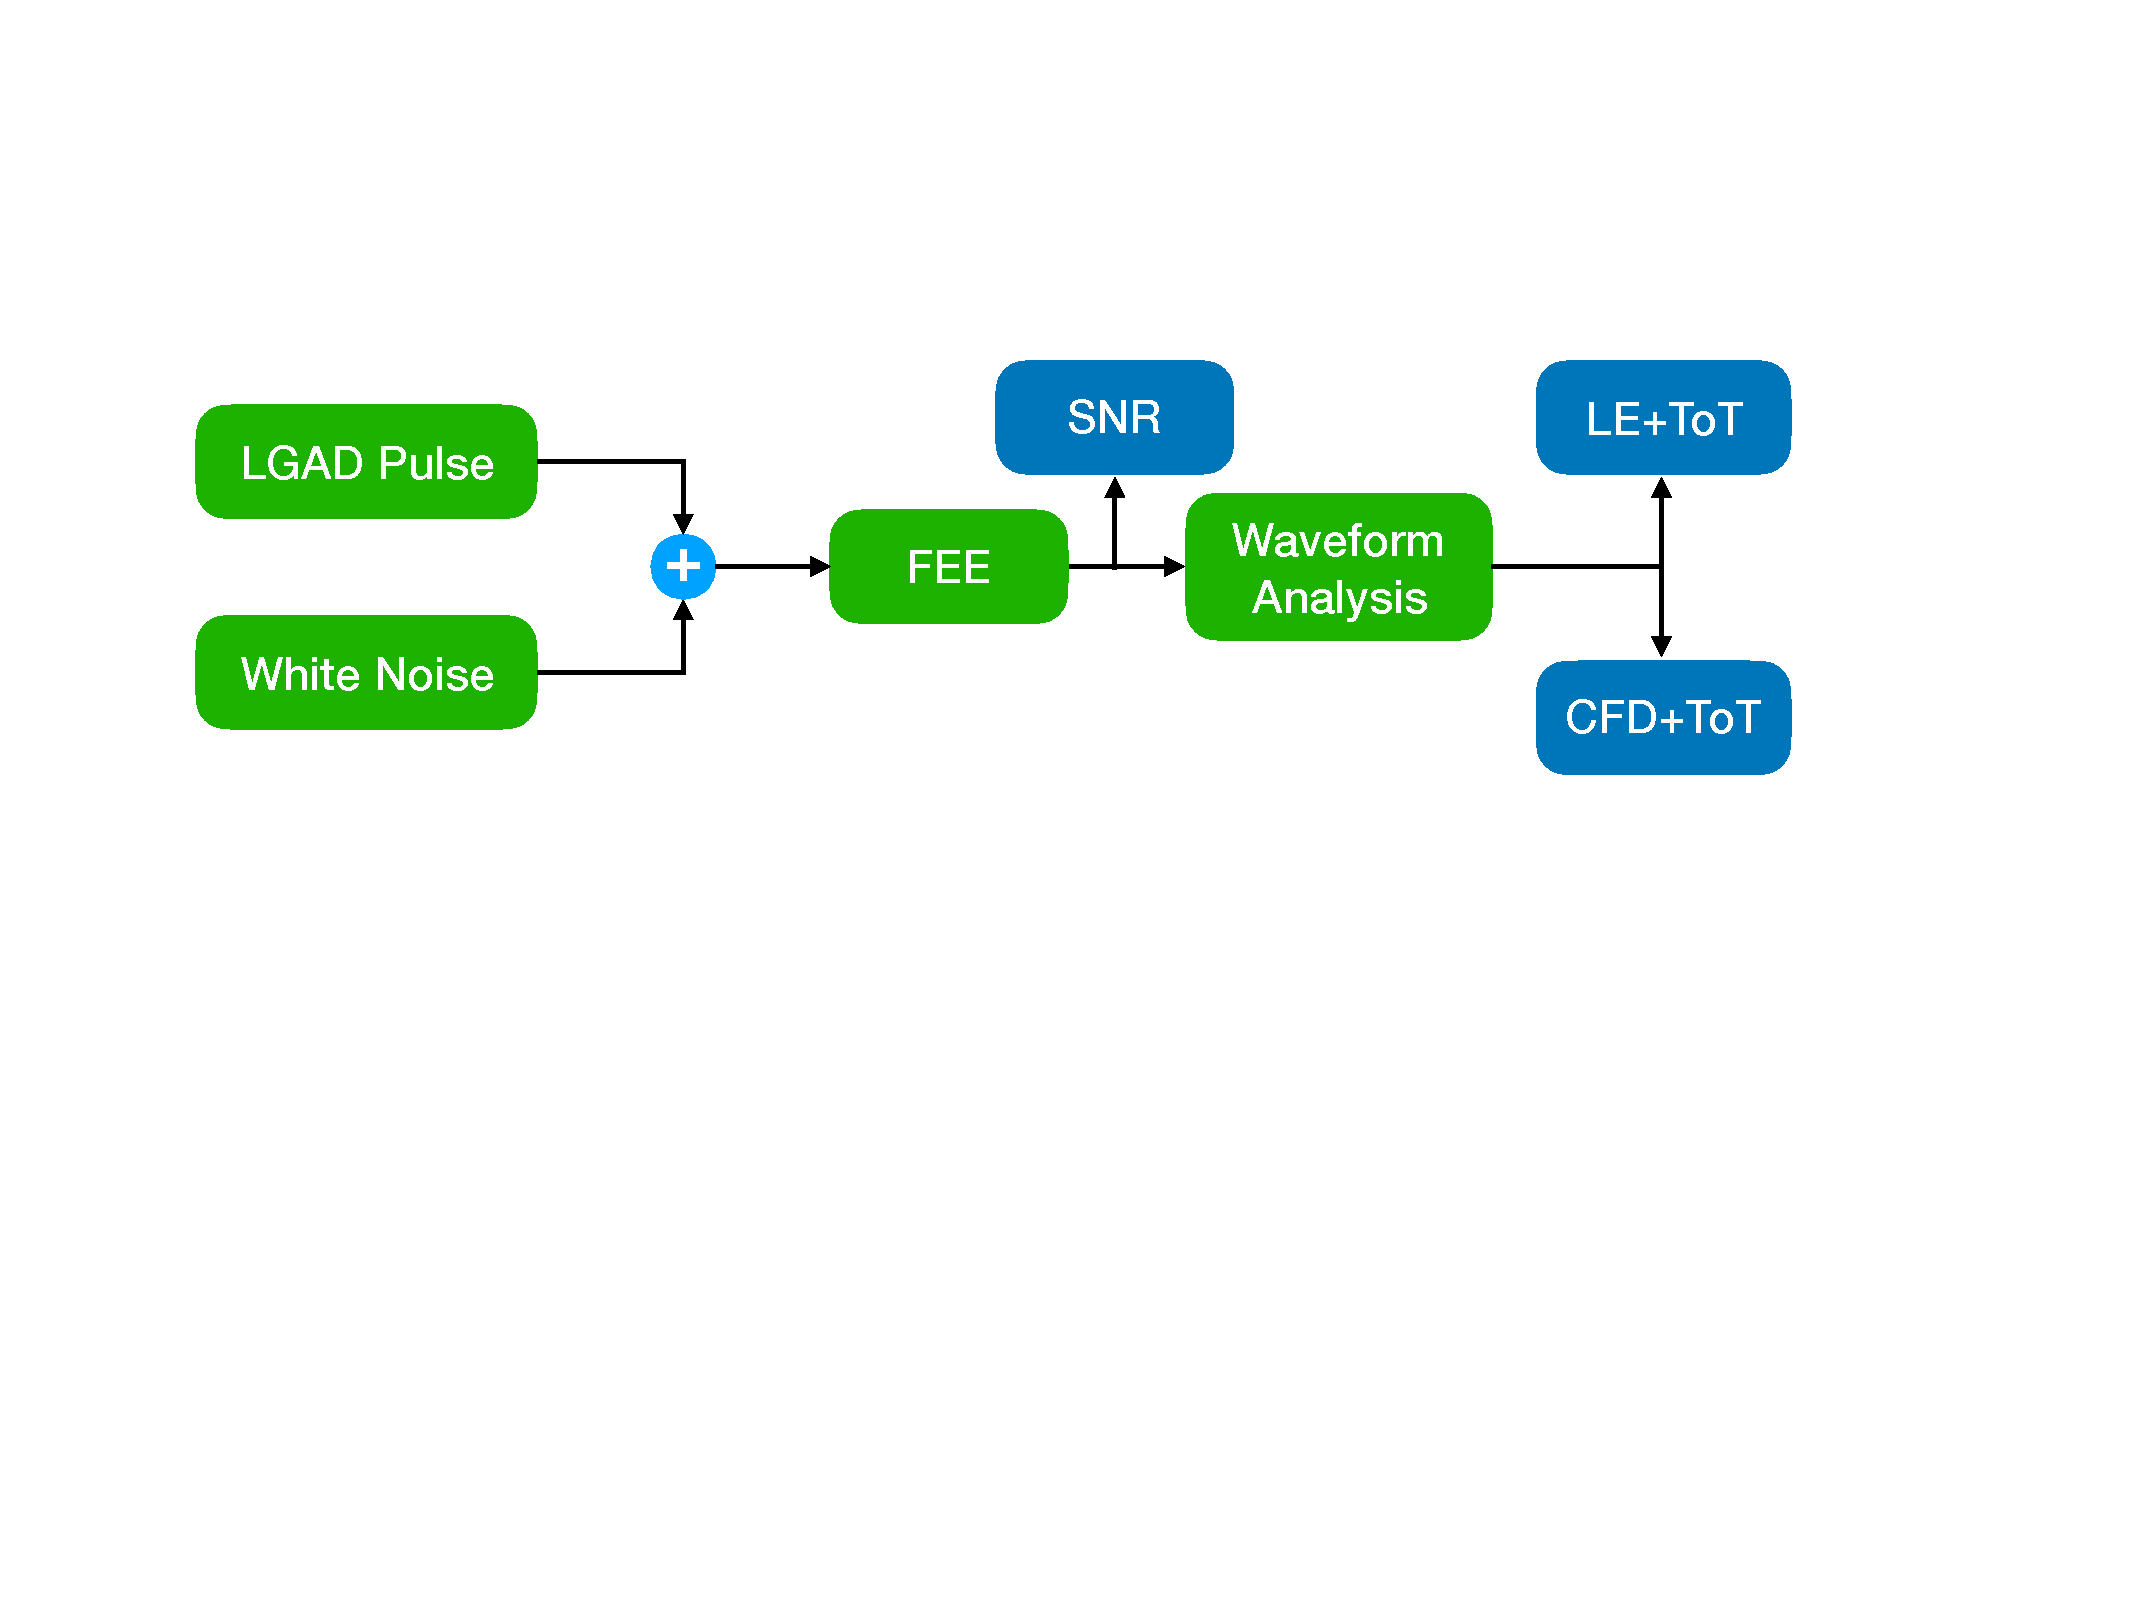
\includegraphics[width=0.75\textwidth]{figs/lgad_simulation_diagram.pdf}
\caption{A schematic diagram of the simulation. Each simulation configurable block is shown in green. The most relevant outputs
of the simulation are shown in blue.}
\label{fig:simulation_diagram}
\end{figure}

%\subsection{LGAD pulse library and simulation}
%\label{sub_sec:lgad_pulse_library}
%e need to ask Nicolo to send us a paragrah for the Weightfield2 (WF2)

\subsection{Front-end electronics and noise injection}
\label{sub_sec:fee_simulation_and_noise}
The front-end simulation combines analytical calculations and
numerical methods. We implement two independent simulations,
one based on the time domain and the other on the Laplace domain. Both simulation use as input
 the unprocessed WF2 LGAD pulses. The results of the two simulations
 are in agreement within statistical uncertainties and provide a cross check of the results.
 Sections~\ref{sec:fee} and~\ref{sec:noise_simulation} describe
the details of the implementation of the front-end and noise simulation.
%We implement most of the calculations in the time domain, while the frequency domain is mostly used
%to cross-check noise and the expected FEE response. Sections~\ref{sec:fee} and~\ref{sec:noise_simulation} describe
%the details of the implementation of the front-end and noise simulation.

\subsubsection{Front-end simulation}\label{sec:fee}
The front-end simulation is based on a single amplification stage. We focus on the BW of such an amplifier rather than variations
thereof. The FEE is a second order low-pass filter with transfer function ($H(S)$)
and impulse response ($h(t)$) given by equations~\ref{eq:filter_tf} and~\ref{eq:filter_ir}, respectively.

 \begin{tabularx}{\textwidth}{XX}
 \begin{equation}\label{eq:filter_tf}
   H(S) = \frac{\frac{1}{\tau_{s}^{2}}}{(S+1/\tau_{s})^{2}}
 \end{equation}
     &
 \begin{equation}\label{eq:filter_ir}
     h(t) = \frac{t}{\tau_s^2}e^{-t/\tau_{s}}
 \end{equation}
 \end{tabularx}\par
%Si: I don't like this tabular way of writing the two equations much...I suggest you just make it two equations in two lines.

The output pulse of the FEE is the convolution (in time domain) of the unprocessed LGAD signal pulse from WF2 and the FEE impulse response
function, given in Eq.~\ref{eq:filter_ir}. The time base for the pulses and the convolution is 10~\si{ps}, and we use this sampling time
throughout the simulation. As stated above we focus the study on the BW of the FEE and to that end we scan the $\tau_{s}$ paremeter
in Eq.~\ref{eq:filter_ir} in the following set:\{0.5, 1, 2, 4\}~\si{ns}. This parameter is hereafter referred to as
shaping time (ST). Figure~\ref{fig:ir_and_lgad} (left) shows the comparison of the impulse and LGAD responses for a ST of 1~\si{ns} while
Figure~\ref{fig:ir_and_lgad} (right) shows the LGAD response for all STs studied. We observe that the LGAD response is delayed with respect
to the impulse response,  and that pulse slew rate is decreased in the first nanosecond of the pulse. As expected, we also observe
that the pulse risetime scale up with the ST and that the decay time is dominated by the ST.
The measured risetimes (10\% to 90\%) are shown in Tab.~\ref{tab:risetime}.
%[Si: what does it mean that decay time is ``dominated'' by ST? Dont' understand that sentence]


\begin{figure}[htbp]
  \centering
  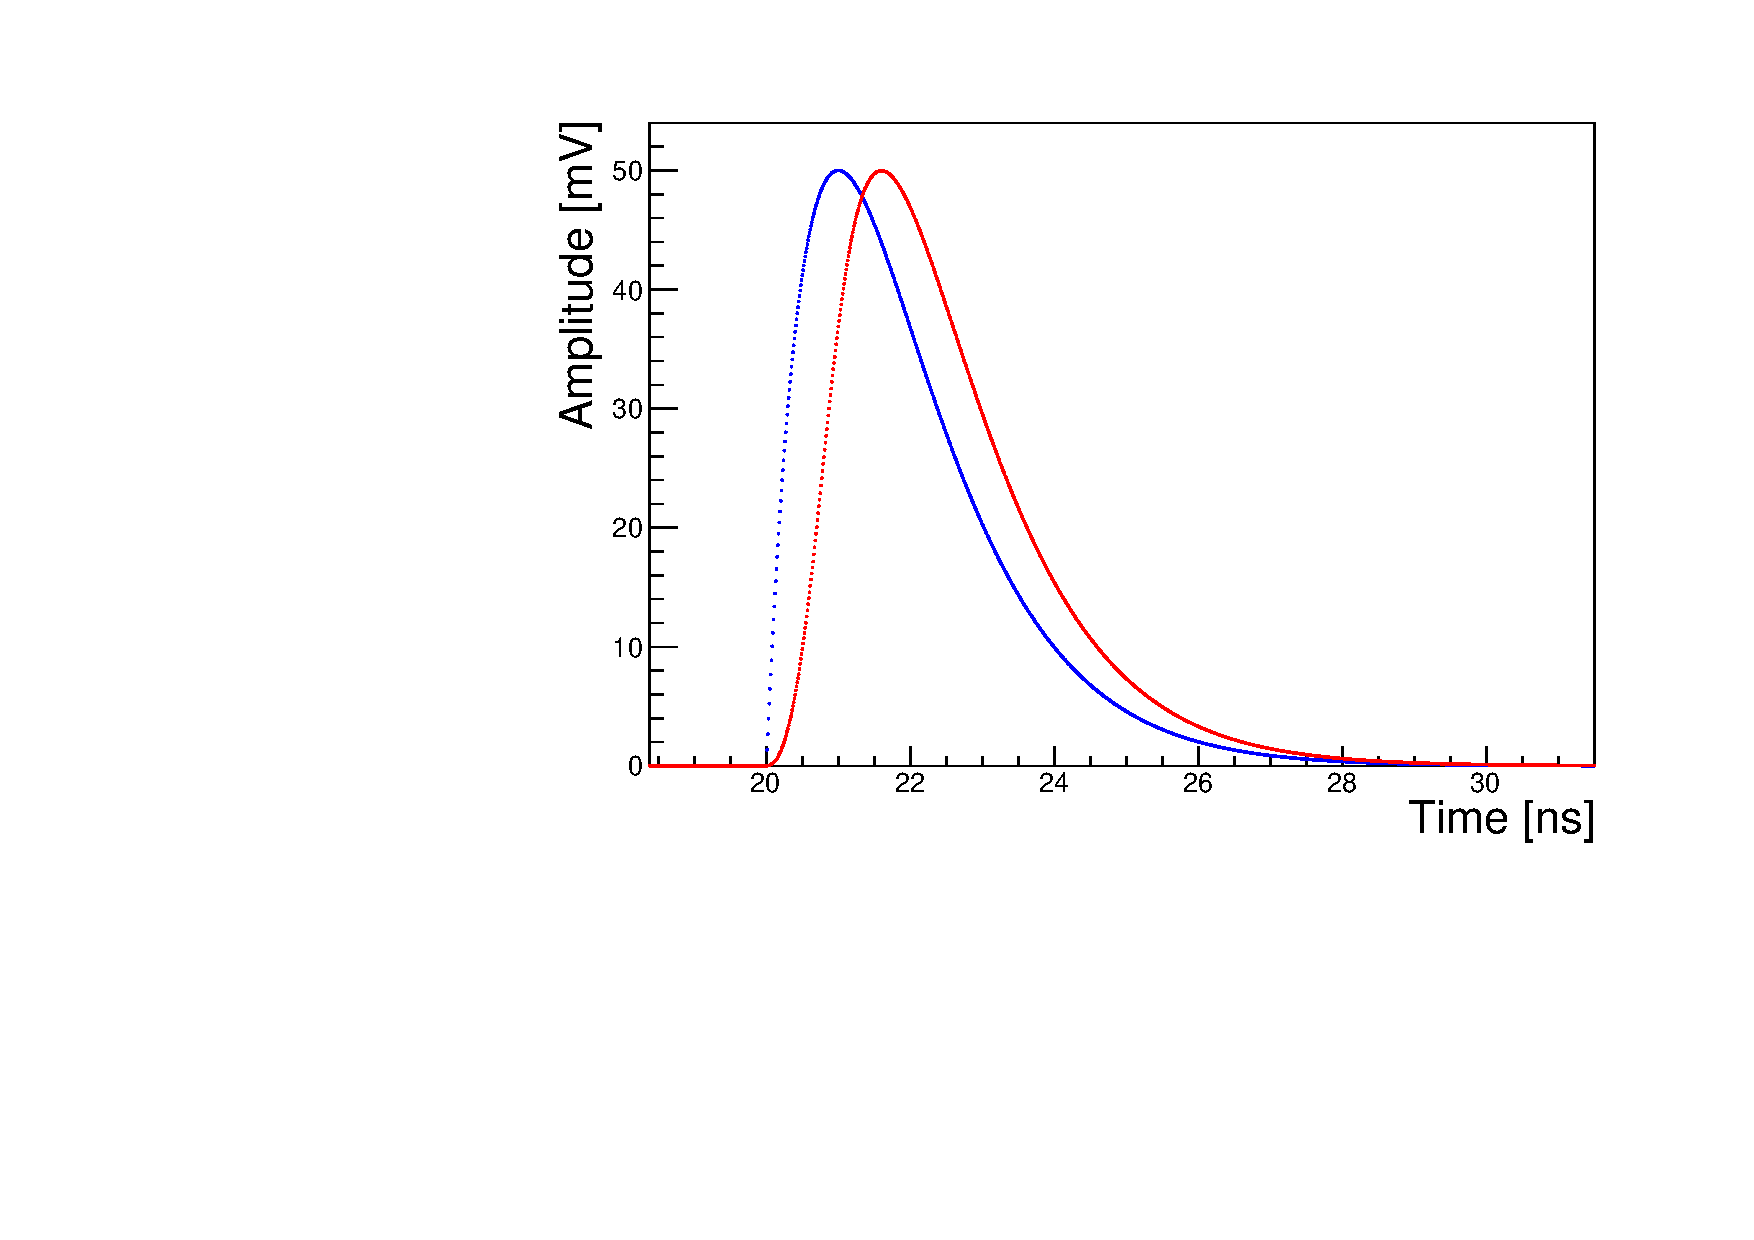
\includegraphics[width=0.48\textwidth]{figs/impulse_vs_lgad_response_1ens_shaping.pdf} \hfill
  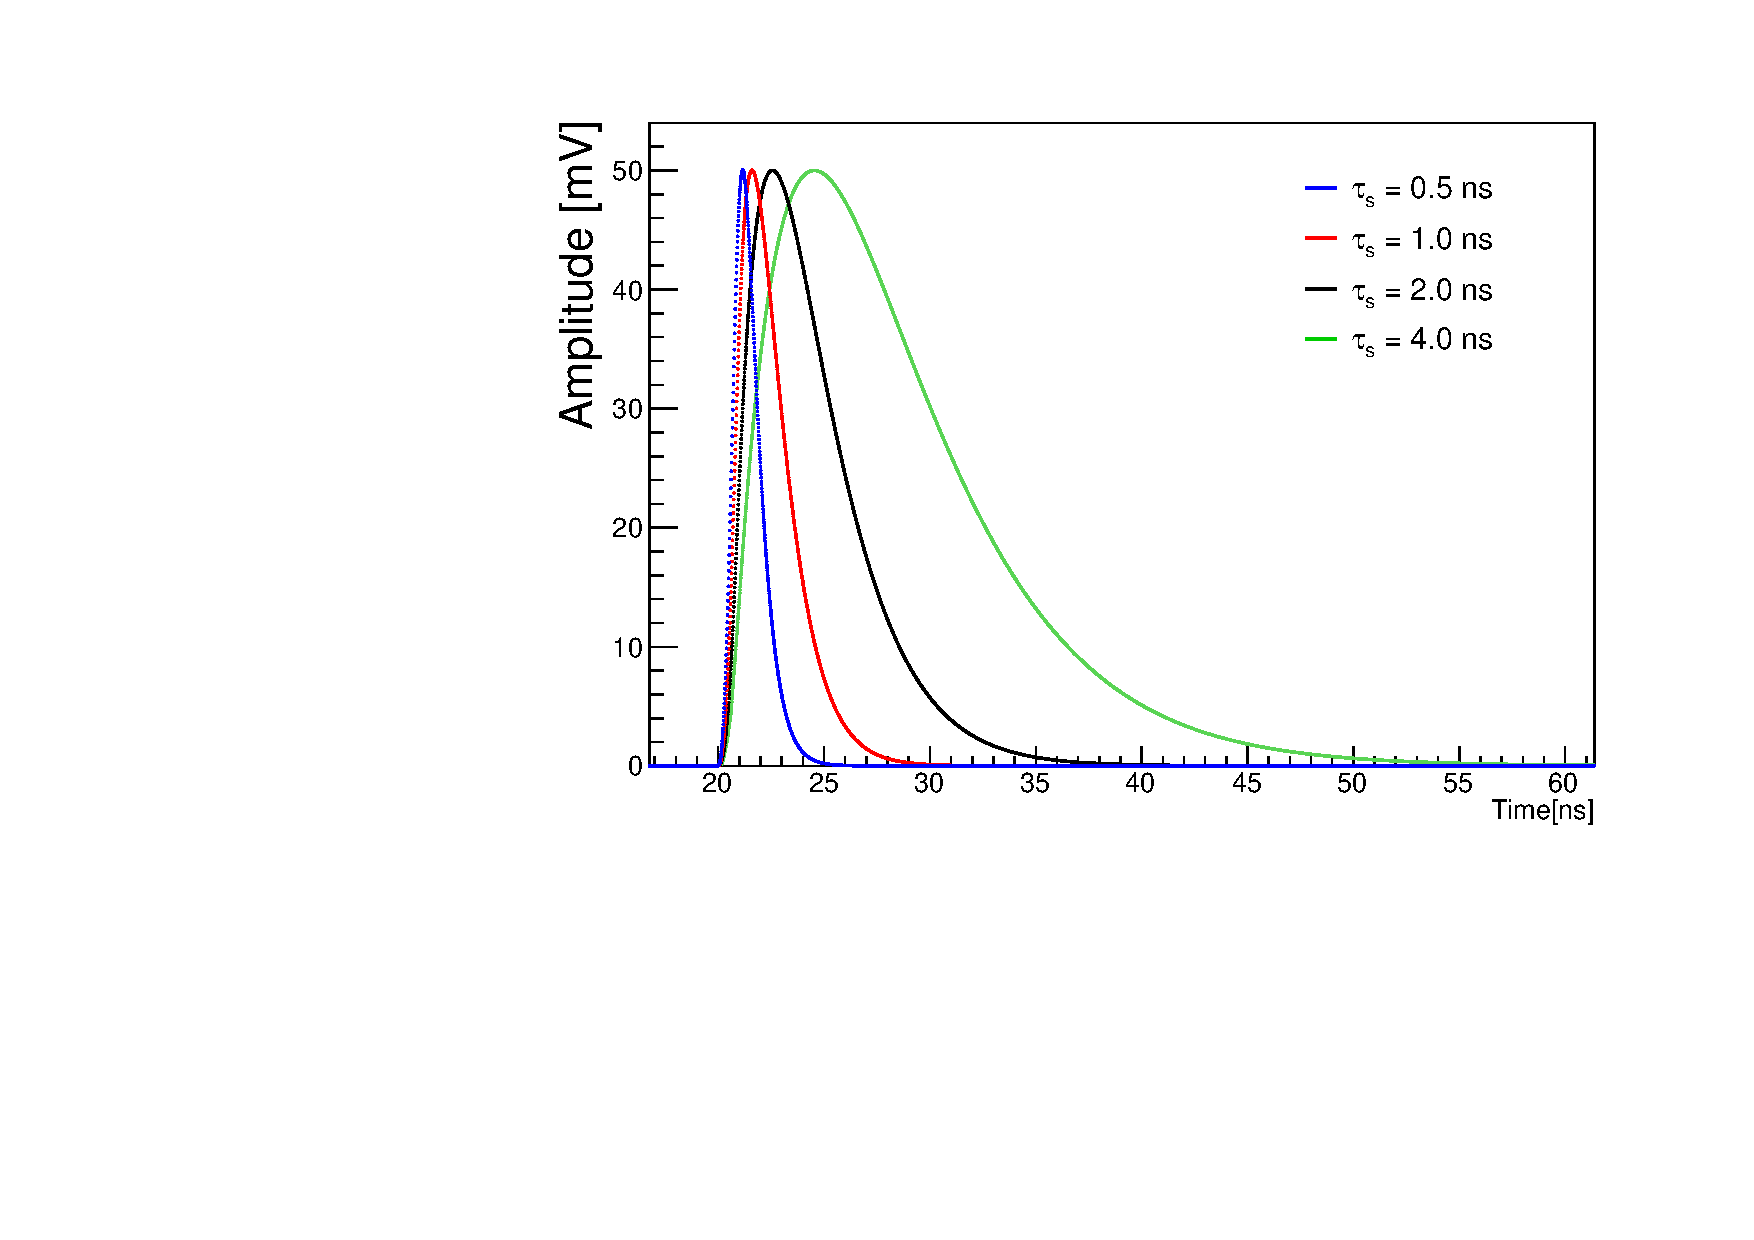
\includegraphics[width=0.48\textwidth]{figs/lgad_all_shaping_time_noiseless.pdf}
  \caption{(Left) Comparison of impulse and LGAD reponses for the a shaping time (ST) of 1~\si{ns}.
  (Right) LGAD response for the four shaping times studied: \{0.5, 1, 2, 4\}~\si{ns}. All pulses have been nomalized
  to achive a peak amplitude of 50~\si{mV}. Legends for the shaping times are shown in the plots.}
  \label{fig:ir_and_lgad}
\end{figure}


\begin{table}\label{tab:risetime}
  \begin{center}
    \begin{tabular}{c|cccc}
    %\multicolumn{1}{c}{}& \multicolumn{4}{c}{Risetime (10-90\%) (ps)} \\
    %\multicolumn{1}{c}{}& \multicolumn{3}{c}{$\mathrm{(RC)}^{2}$ Constant Fraction}\\ \hline
    ST (ns) & 0.5  & 1.0 & 2.0 & 4.0 \\\hline
    Risetime (ns) & $0.7\pm xx$ & $0.9\pm xx$ & $1.4\pm xx$ & $2.5\pm xx$ \\
    \end{tabular}
    \caption{Measured risetime for all shaping times studied: \{0.5, 1, 2, 4\}~\si{ns}. Risetime is the $10\% - 90\%$ time
    difference as measured by the CFD algorithm described in Sec.~\ref{sec:le_and_cfd}.}
  \end{center}
 \end{table}

%Si: What are the uncertainties ``xx''?



\subsubsection{Noise injection}\label{sec:noise_simulation}
Gaussian white noise is simulated by sampling the full time window (0 - 100~\si{ns}) in 10~\si{ps} intervals. Each
sampled time is assign a random amplitude which is drawn from a gaussian distribution with zero mean and width corresponding to the SNR
under study. It is important to note that the width of the gausian parameter is not exactly the SNR and needs to be adjusted depending
on the ST of the FEE. The left panel of Figure~\ref{fig:noise} shows the gaussian white noise before and after a 1~\si{ns} FEE.
The expected behavior for the noise is observed. The left panel of Figure~\ref{fig:noise} shows the output of the
FEE block, with a 1~\si{ns} ST, for a pre-irradiated LGAD pulse after noise has been injected. The injected noise is
such that the SNR is 30. SNR is defined ratio of the landau peak (the most probable value or MPV) of the pulse height distribution to the
the r.m.s of the 100th sample over an ensemble of 1000 pulses.

\begin{figure}[htbp]
  \centering
  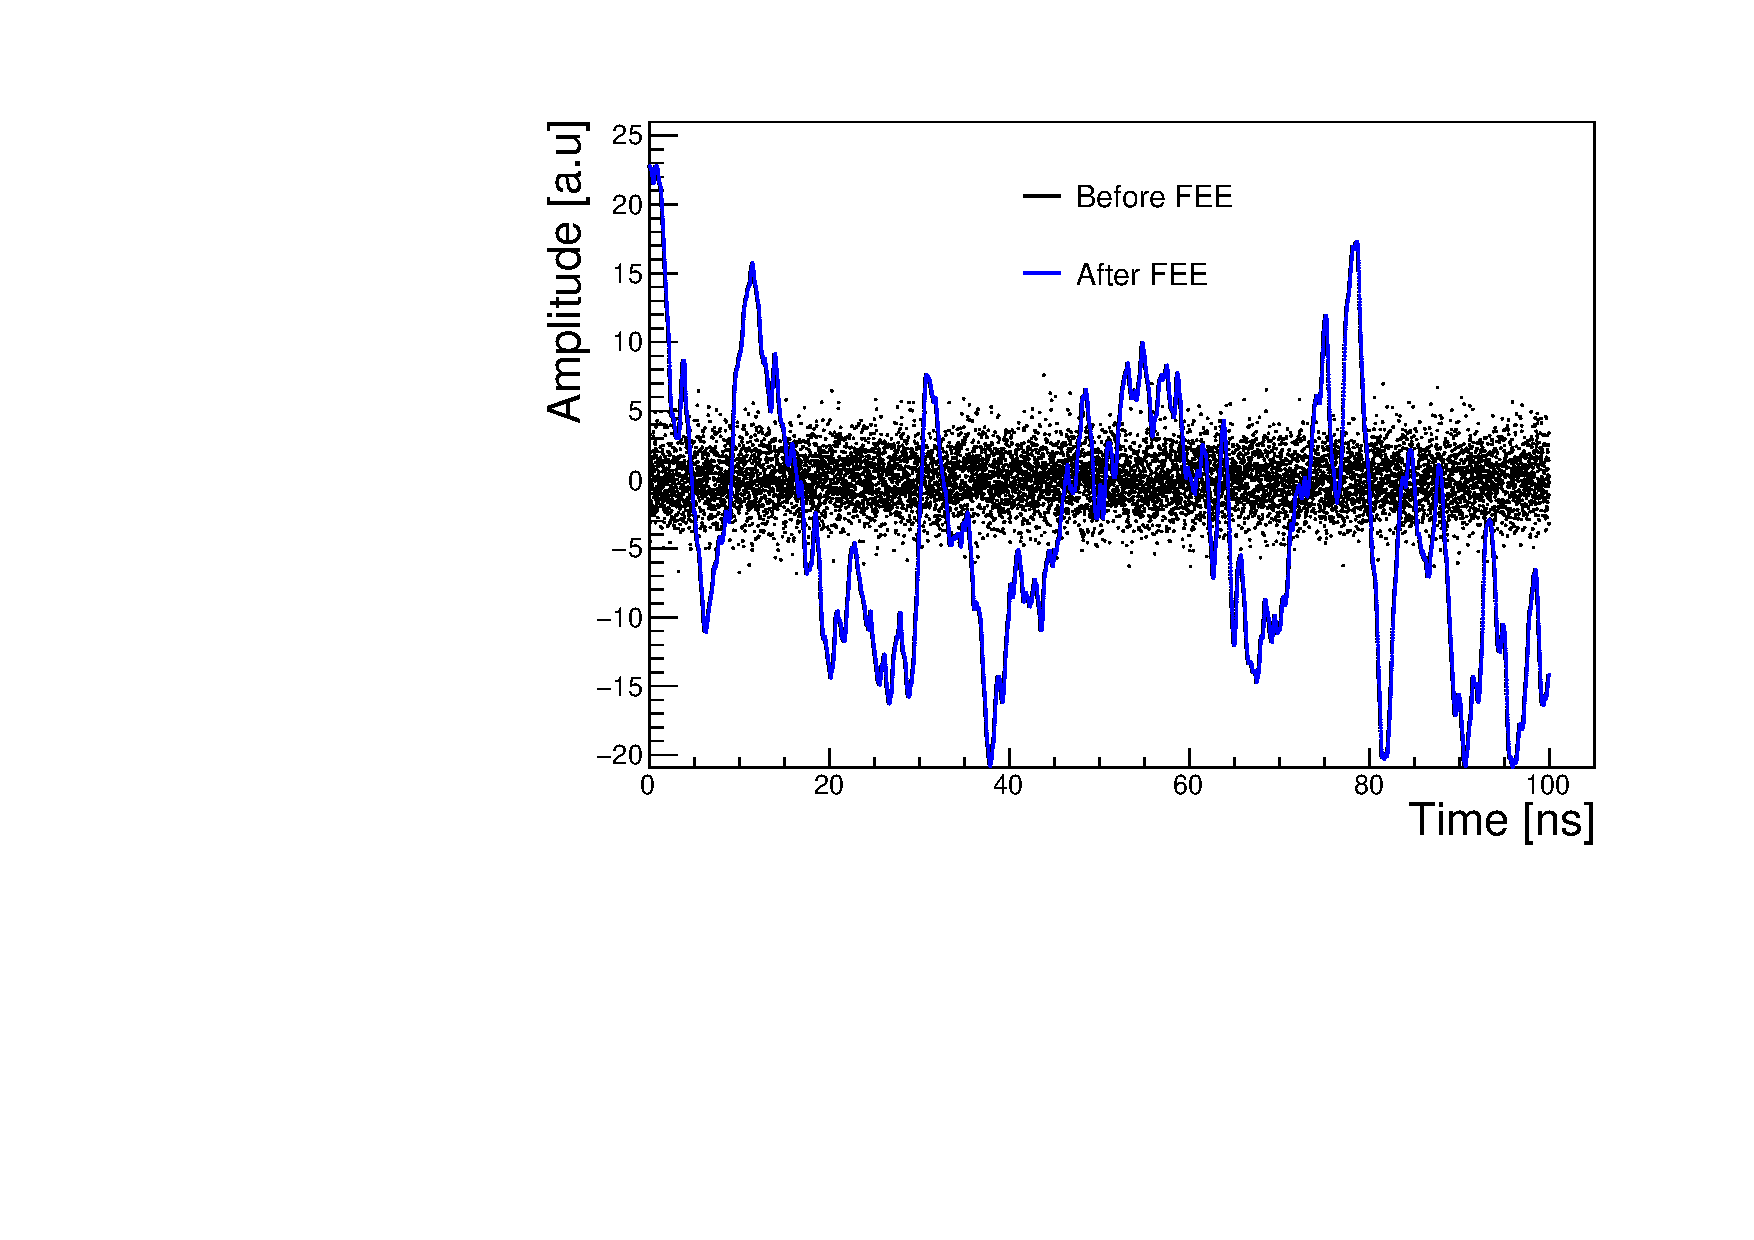
\includegraphics[width=0.48\textwidth]{figs/noise_vs_shaped_noise.pdf} \hfill
  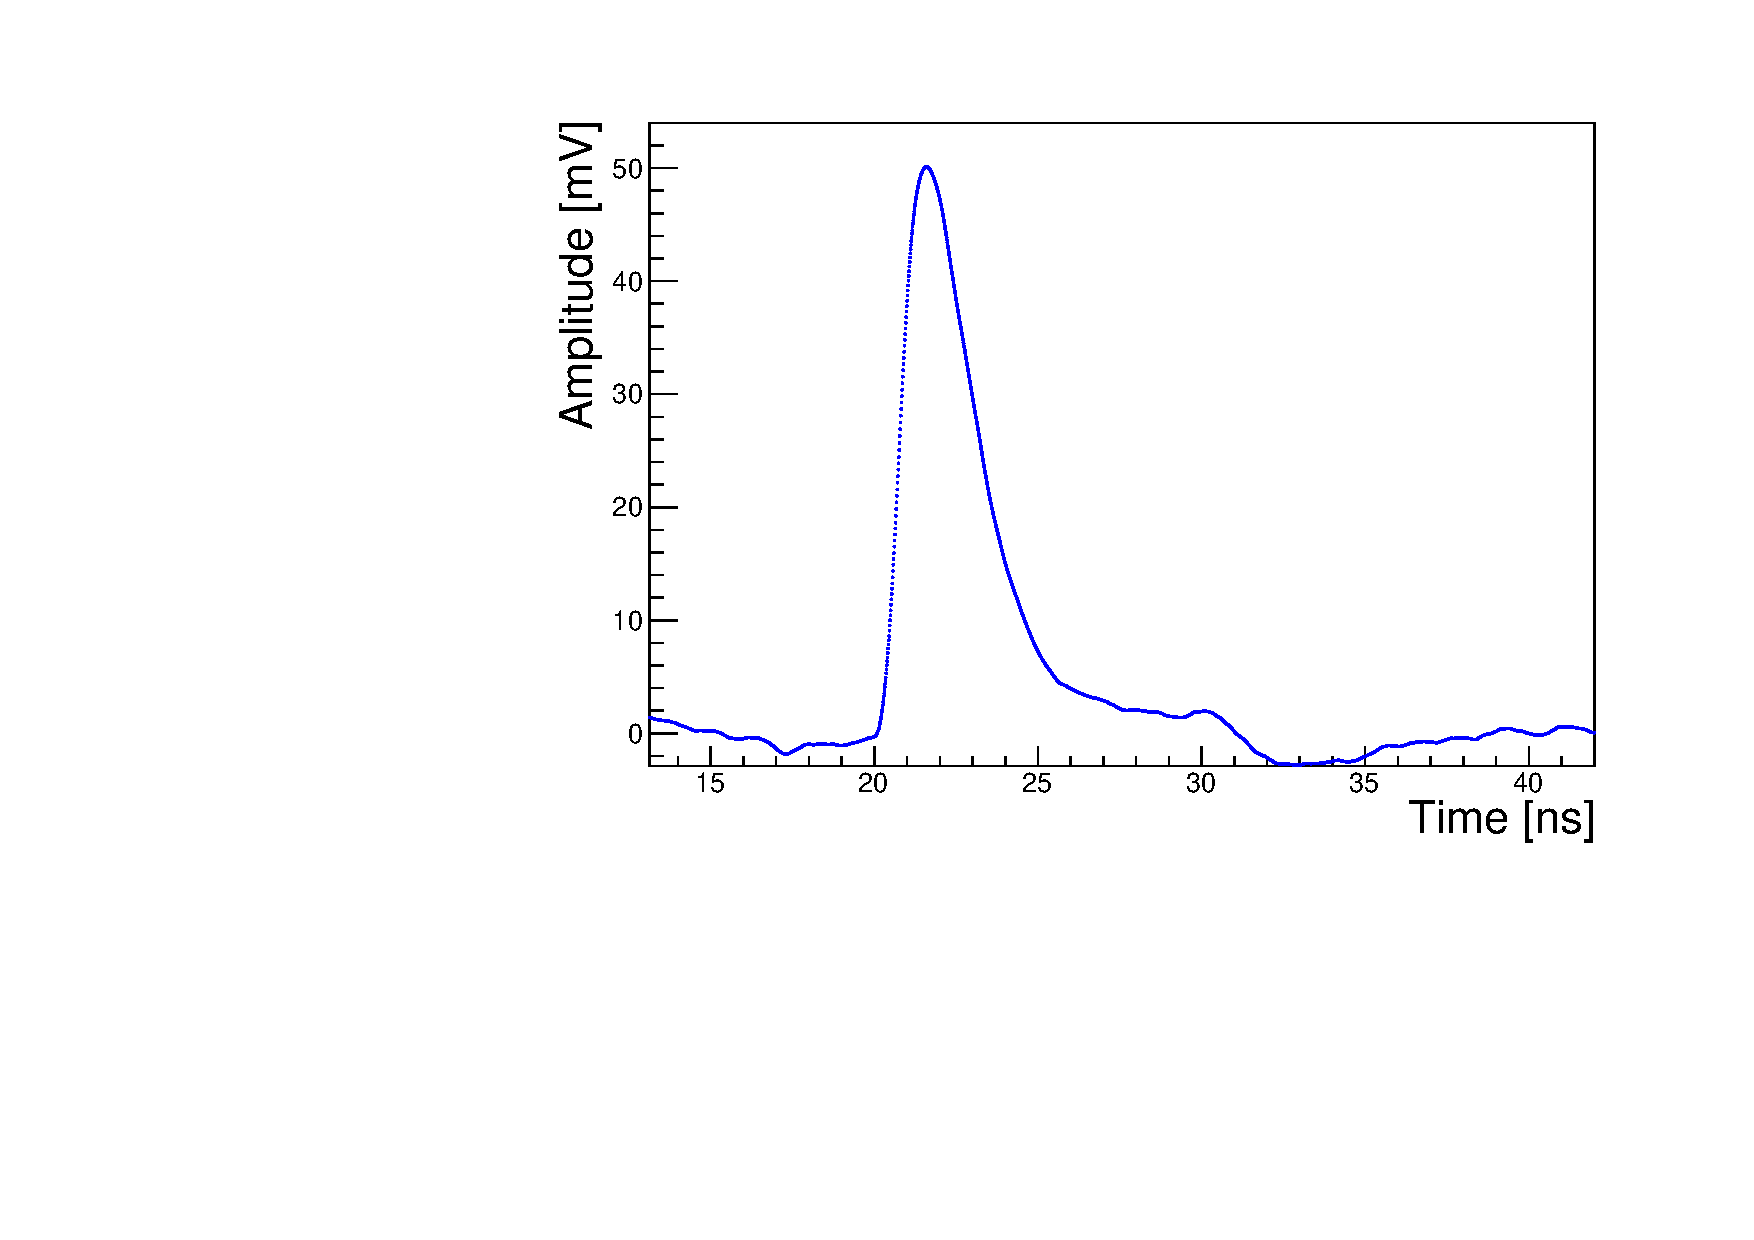
\includegraphics[width=0.48\textwidth]{figs/lgad_pre_rad_st_1ns_snr_30.pdf}
  \caption{(Left) Comparison of gaussian white noise before and after the FEE.
  (Right) Example pulse at the output of the FEE block with a SNR of 30. Both figure use a shaping time (ST) of 1~\si{ns}. Legends for the shaping times are shown in the plots.}
  \label{fig:noise}
\end{figure}

\section{Timing Reconstruction and Analysis}\label{sec:timing_and_analysis}
The time reconstruction is based on waveform analysis. We generate an ensamble of 1000 pulses sampled every 10 ps.
Each pulse is interpolated using the Whittaker-Shannon formula (sin(x)/x). Using the interpolated pulse we assign a timestamp by finding when
a given voltage threshold has been crossed. The threshold can be a constant value (LE) or a constant fraction
 of the pulse height (CF).
In the case of the CFD we also simulate more \textit{realistic} implementations:{\color{red}split-and-delay as well as asecond order RC filter (Greg, please check naming)}.
 More details about the algorithms are given in Sec.~\ref{sec:le_and_cfd}. The time resolution is estimated by the width parameter
of a gaussian fit to the timestamps obtained for a particular theshold. We apply a time-walk correction based on the
time-over-threshold of the pulse. We note that this correction has a large improvement on the time resolution measured
using the LE algorithm while the CF algorithm is mostly insentive to this correction, as seen in Fig.~\ref{fig:time_resolution_scan}.
Details about this correction are covered in Sec.~\ref{sec:tw_and_tot}. The timestamps are measured with a
20~\si{ps} binning while the time-over-thershold is measured with a 100~\si{ps} binning in order to simulate the effect of time quantization.
We scan the LE and CF threshold such that we find the one with the lowest jitter.

\subsection{Leading edge and constant fraction discriminators}\label{sec:le_and_cfd}
The leading edge and constant fraction discriminator algorithms are \textit{ideal} in the sense that they don't simulate the effect of
electronics in a real implementation. Our approach is to sample the pulses every 10~\si{ps} and subsequently interpolate them
using the Whittaker-Shannon formula (sin(x)/x) to more accurately determine the threshold crossing. In the LE case the theshold is scanned
from 3--60~\si{mV}, while the CFD is scanned from 5--90~\% of the current pulse maximum amplitude. For each thershold we obtain two
timestamps: when the pulse first crosses the threshold ($t_{0}$) and when it crosses the second time ($t_{1}$), now in the opposite
direction. The time-over-threshold is defined as the difference of the two timestamps ($\mathrm{ToT} = t_{1} - t_{0}$). The first
timestamp, $t_{0}$, is used to determine the time resolution at given threshold. The time resolution is defined as the width of
a gaussian fit to the $t_{0}$ distribution binned with a bin-width of 20~\si{ps}. The time resolution is obtained in two cases:
before and after a time-walk correction. The time-walk correction aims to correct the known effect of time drift as a function
of the pulse height. The time-walk correction removes this time drift and ensures that the time response is flat as a function
of the pulse height. It is explained in greater detail in Sec.~\ref{sec:tw_and_tot}.
Figure~\ref{fig:time_resolution_scan} shows the time resolution as a function
of the threshold required for a pre-irradiated LGAD sensor with a ST of 1~\si{ns} and a SNR of 30.
We note that the effect of the time-walk correction is large for LE and almost negligible for CF.
Fig.~\ref{fig:time_res} shows a typical $t_{0}$ distribution, using the LE and CF algorithms, for the pre-irradiated
LGAD sensor after the ToT correction has been applied. The time resolution ($\sigma_{t}$) is measured to be $37.3 \pm 1.4 $
and $33.0 \pm 1.4$ for the LE and CF, respectively. Additionally, we study the impact of a more \textit{realistic} CFD implementations:
{\color{red}split-and-delay as well as a second order RC filter (Greg, please check naming)} (see Sec.~\ref{sed:cfd_realistic}).
 We observe that \textit{ideal} and split-and delay CFD implementations yield equivalent results within uncertainties.
 The second order RC filter shows a degradation on performance with respect to the split-and delay implementation.

\subsubsection{constant fraction discriminator implementations}\label{sed:cfd_realistic}
{\color{red}GREG: PLEASE ADD TEXT HERE, I called the two implementations split-and-delay and second order RC previousluy in the text (also in red)}.


  \begin{figure}[htbp]
    \centering
    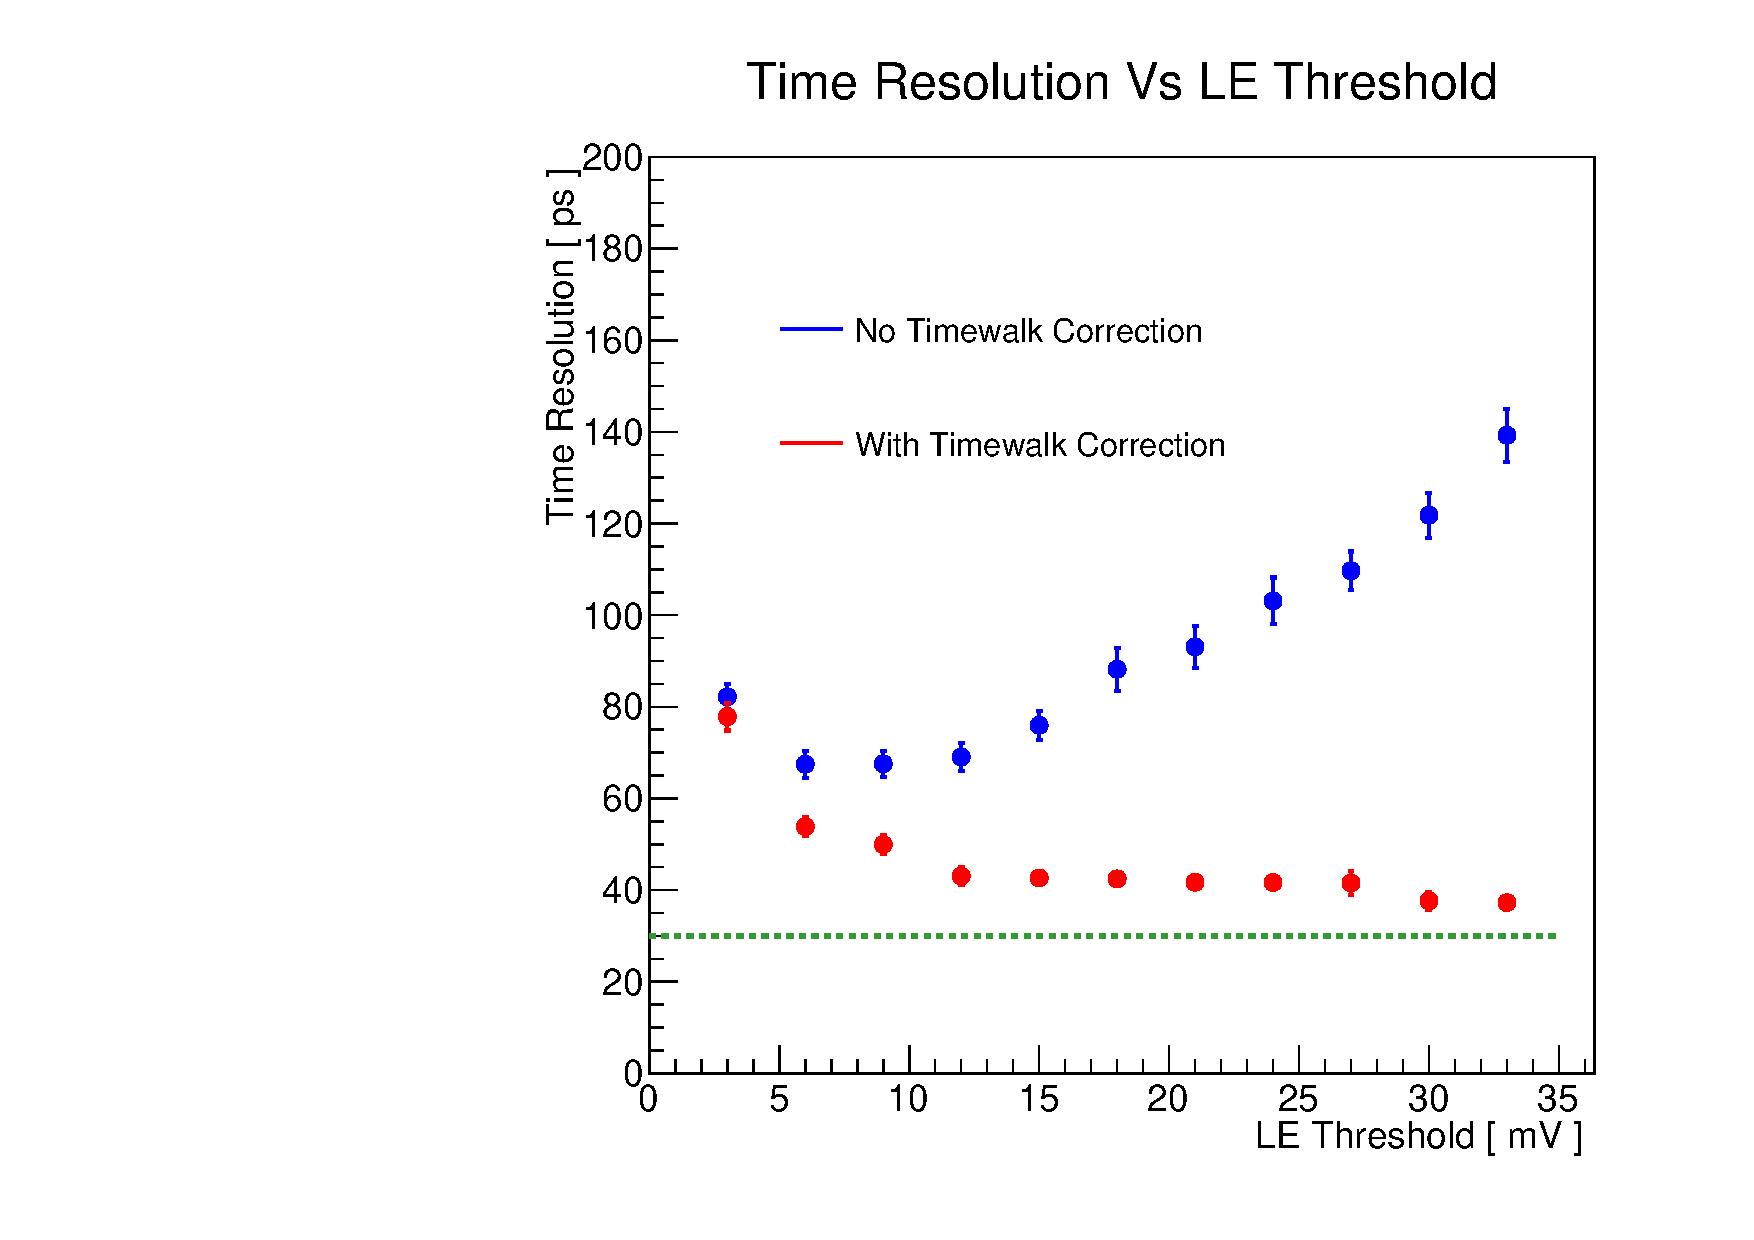
\includegraphics[width=0.48\textwidth]{figs/ShapingTime1p0_SNR30_55MicronGain15Prerad_FIXED_NOISE_FIXED_SNR_V2_converted_TimeResolutionVsThresholdToT.pdf} \hfill
    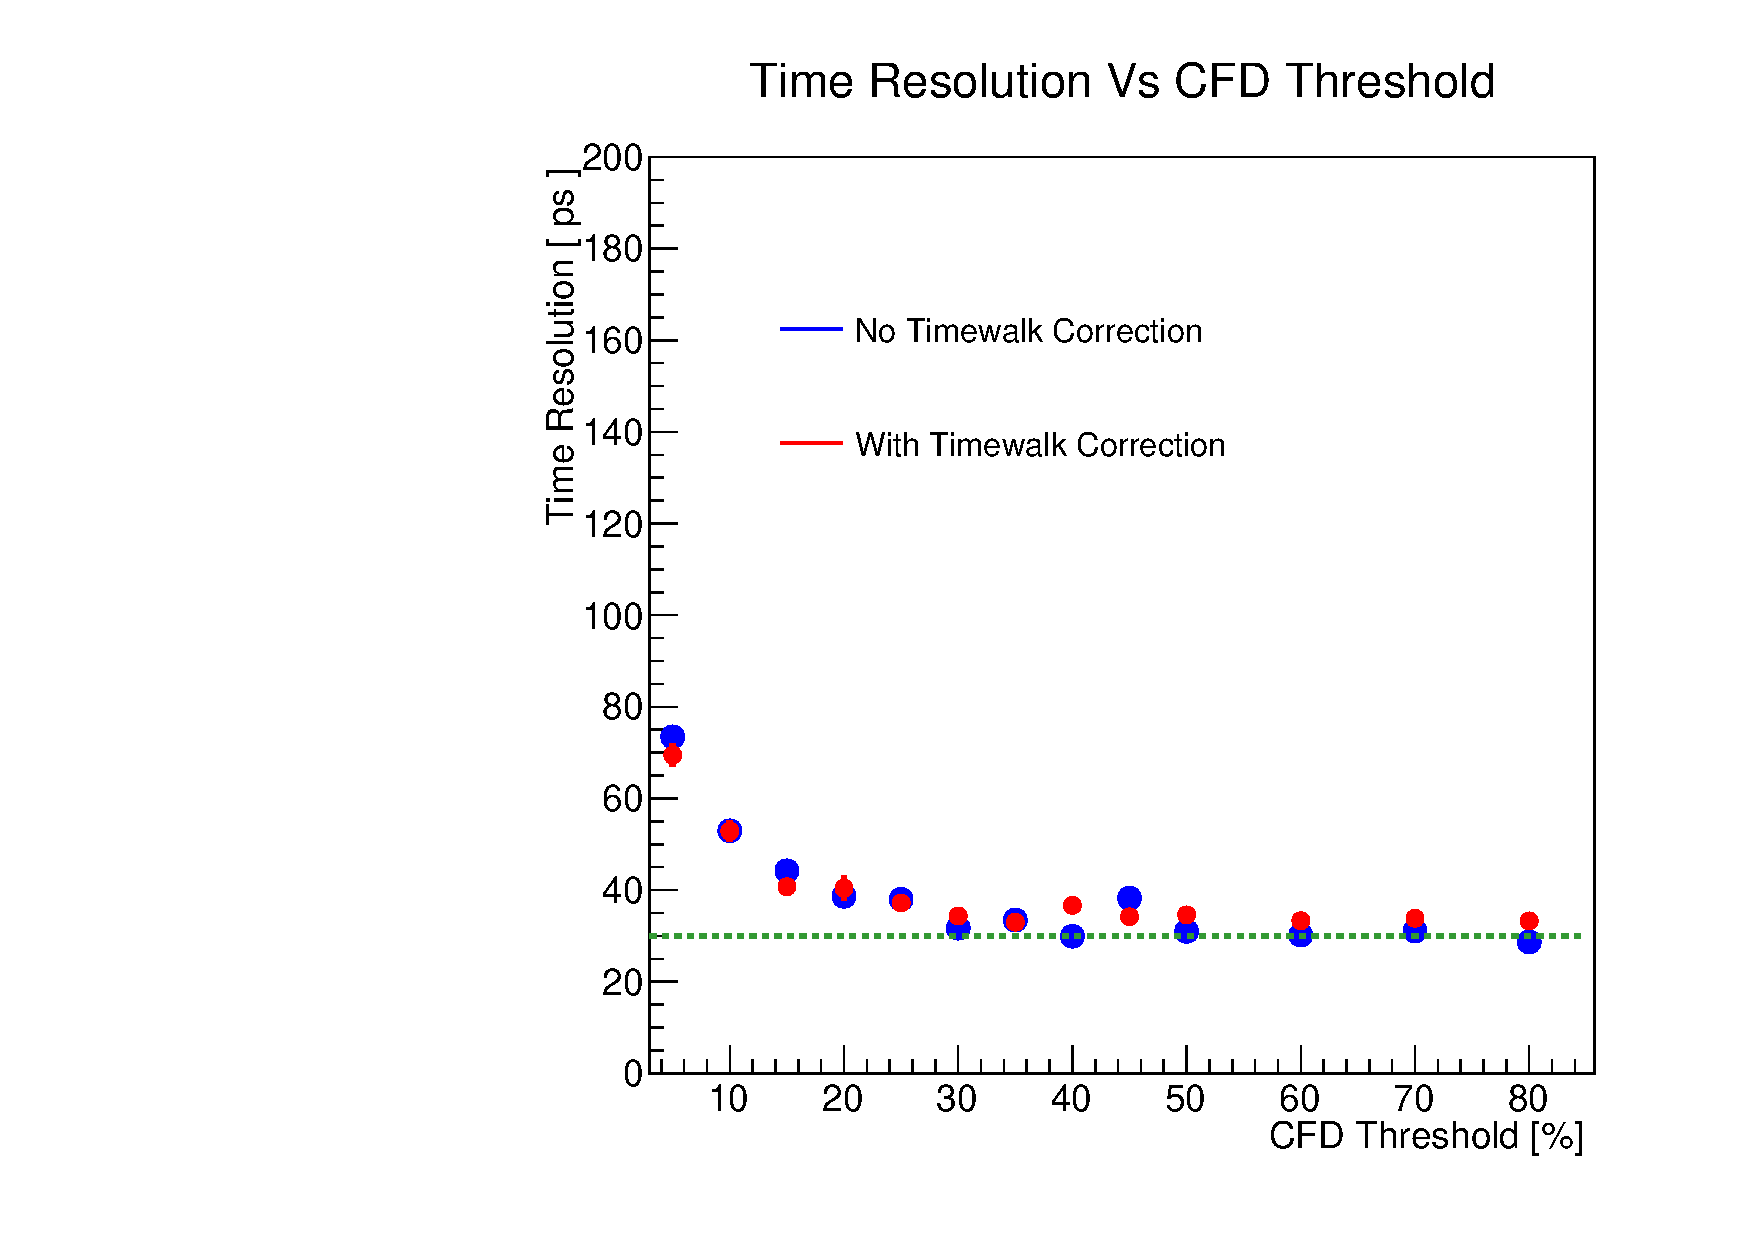
\includegraphics[width=0.48\textwidth]{figs/ShapingTime1p0_SNR30_55MicronGain15Prerad_FIXED_NOISE_FIXED_SNR_V2_converted_TimeResolutionVsThresholdCFD.pdf}
    \caption{(Left) Comparison of gaussian white noise before and after the FEE.
    (Right) Example pulse at the output of the FEE block with a SNR of 30. Both figure use a shaping time (ST) of 1~\si{ns}. Legends for the shaping times are shown in the plots.}
    \label{fig:time_resolution_scan}
  \end{figure}

  \begin{figure}[htbp]
    \centering
    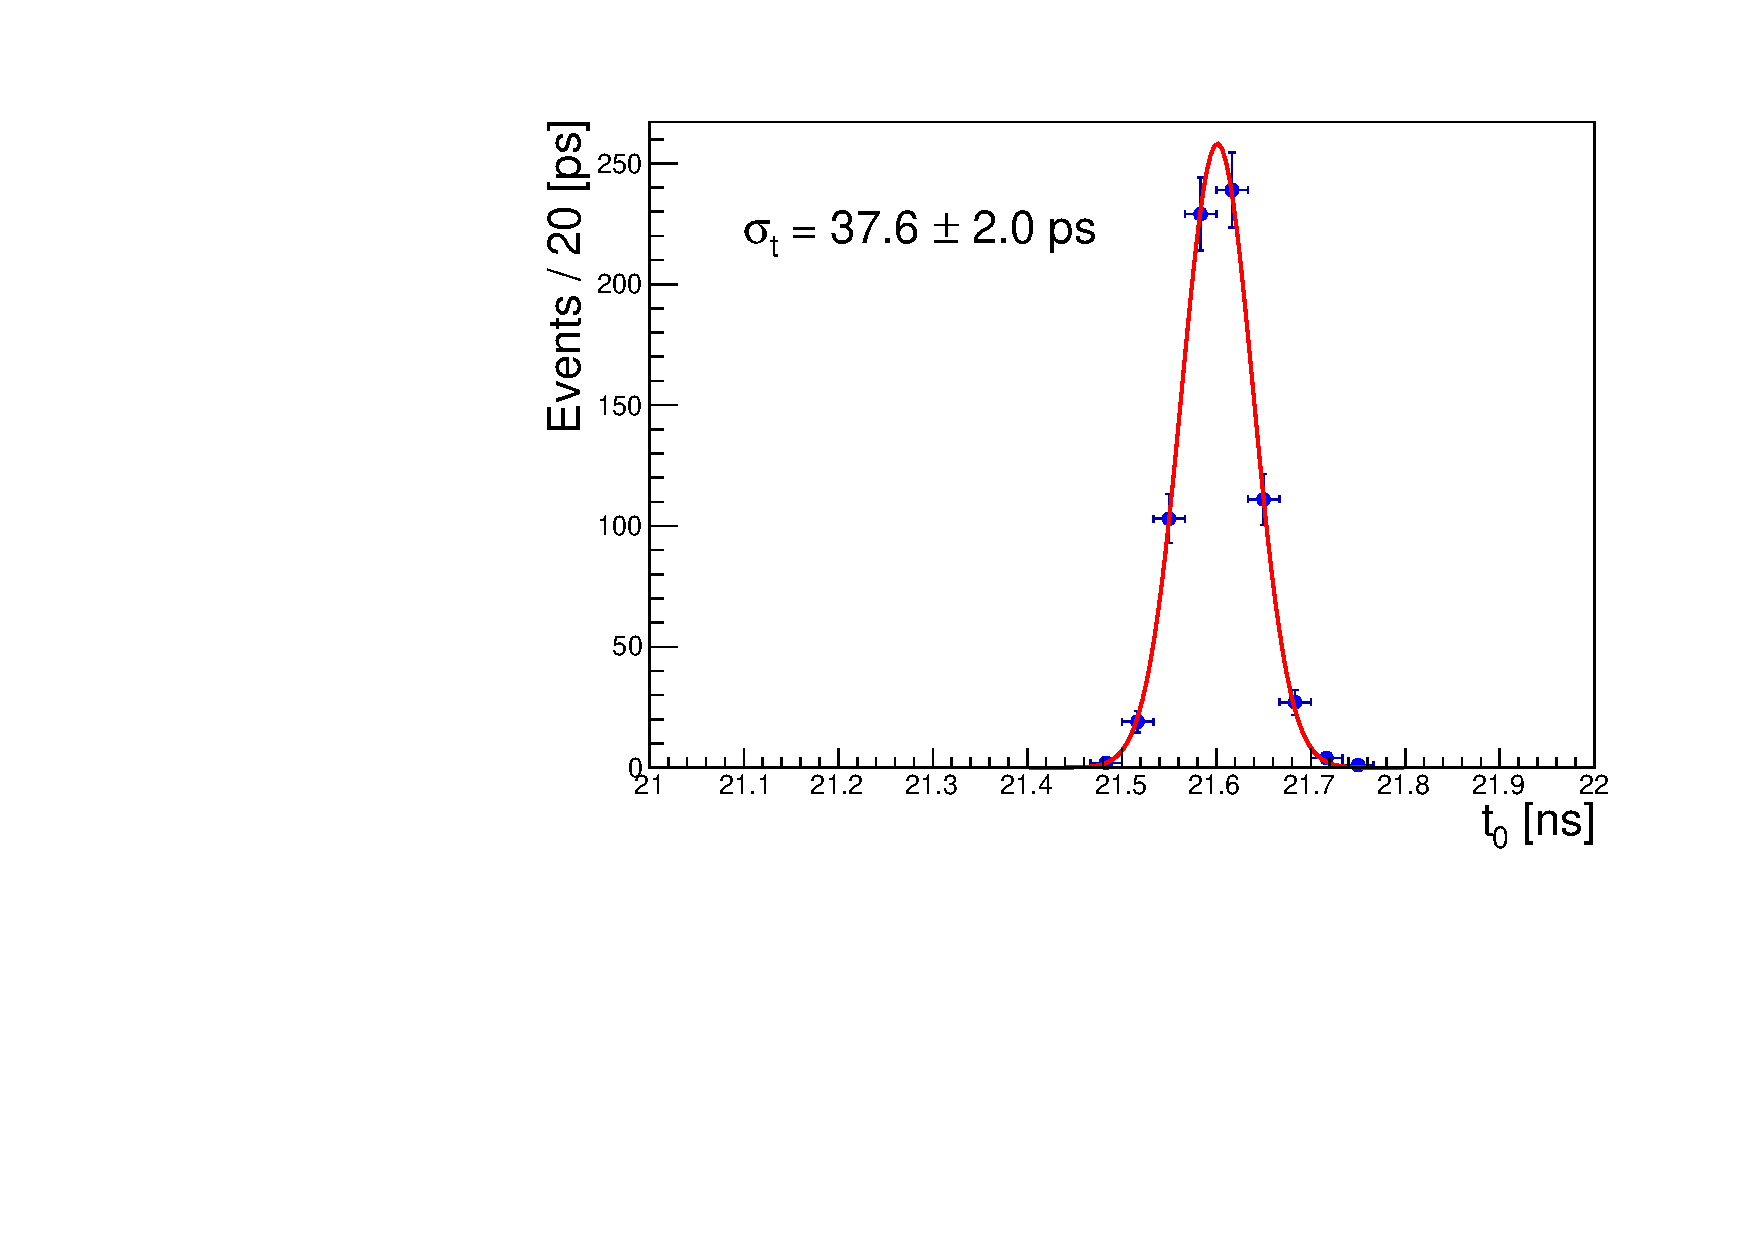
\includegraphics[width=0.48\textwidth]{figs/pre_rad_st_1ns_snr_30_le_tot_threshold_30mV.pdf} \hfill
    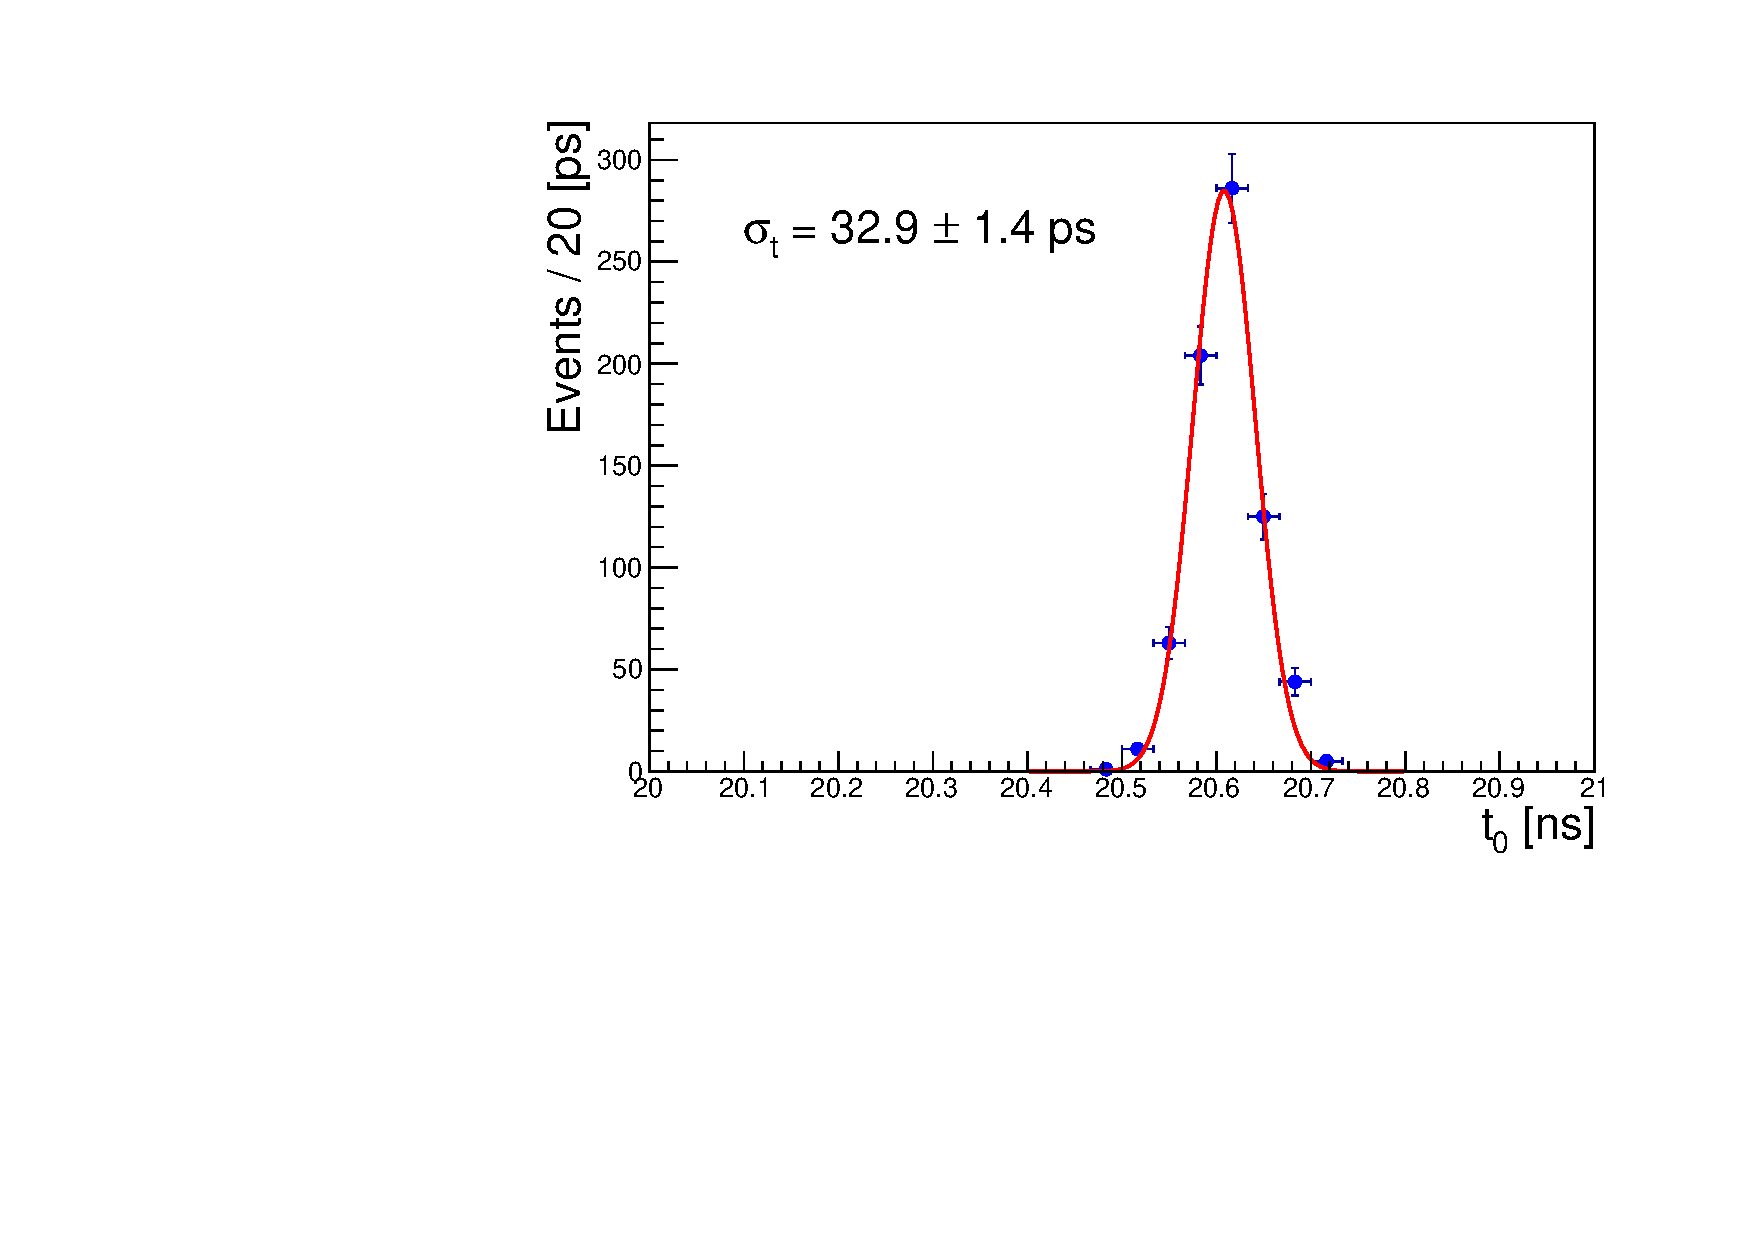
\includegraphics[width=0.48\textwidth]{figs/pre_rad_st_1ns_snr_30_cfd_tot_threshold_35_percent_v2.pdf}
    \caption{(Left) timestamp ($t_{0}$) distribution for a 30~\si{mV} threshold using a leading edge discriminator.
    (Left) timestamp ($t_{0}$) distribution for a 35\% threshold using a constant fraction discriminator. Both figures
    include the time-walk correction based on the measured ToT.
    Both figures use a shaping time (ST) of 1~\si{ns} and correspond to SNR of 30.}
    \label{fig:time_res}
  \end{figure}


\subsection{Time-walk correction and time-over-threshold}\label{sec:tw_and_tot}
A time-walk correction is applied in order to correct the timestamp drift when dealing with pulses of varying amplitudes.
The correction is based on the measured time-over-theshold: $\mathrm{ToT} = t_{1} - t_{0}$. As expected, we observe that the ToT correction
is large for the LE case and negligible for CF (see Fig.~\ref{fig:time_resolution_scan}).
Figure~\ref{fig:ToT} (left) shows a typical two dimensional map of $t_{0}$ and ToT for the
LE algorithm, wherein a clear correlation between $t_{0}$ and ToT is observed. The time-walk correction is obtain by measuring the average
$t_{0}$ in each ToT bin and subsequently fitting a 2nd-order polinomial (see Fig.~\ref{fig:ToT} (right)).
The resulting analytical expression after the fit is then used to correct and flatten the dependence of $t_{0}$ on ToT.
The time-walk correction is expressed in Eq.~\ref{eq:time_walk}, where $p_{2}$ and $p_{1}$ are the quadratic
and linear coefficients of the 2nd-oder polynomial fit. Different corrections are derived for each simulation scenario
characterized by the values of the simulation parameters: ST, SNR, and LGAD irradiation level.
As shown in Fig.~\ref{fig:time_resolution_scan} (left) the effect of the time-walk dependes on the threshold used and correcting for it
can yield significant improvements in the measured time resolution.

\begin{equation}\label{eq:time_walk}
  t_{0} = t_{0}-(p_{2}\mathrm{ToT}^2+p_{1}\mathrm{ToT})
\end{equation}

\begin{figure}[htbp]
  \centering
  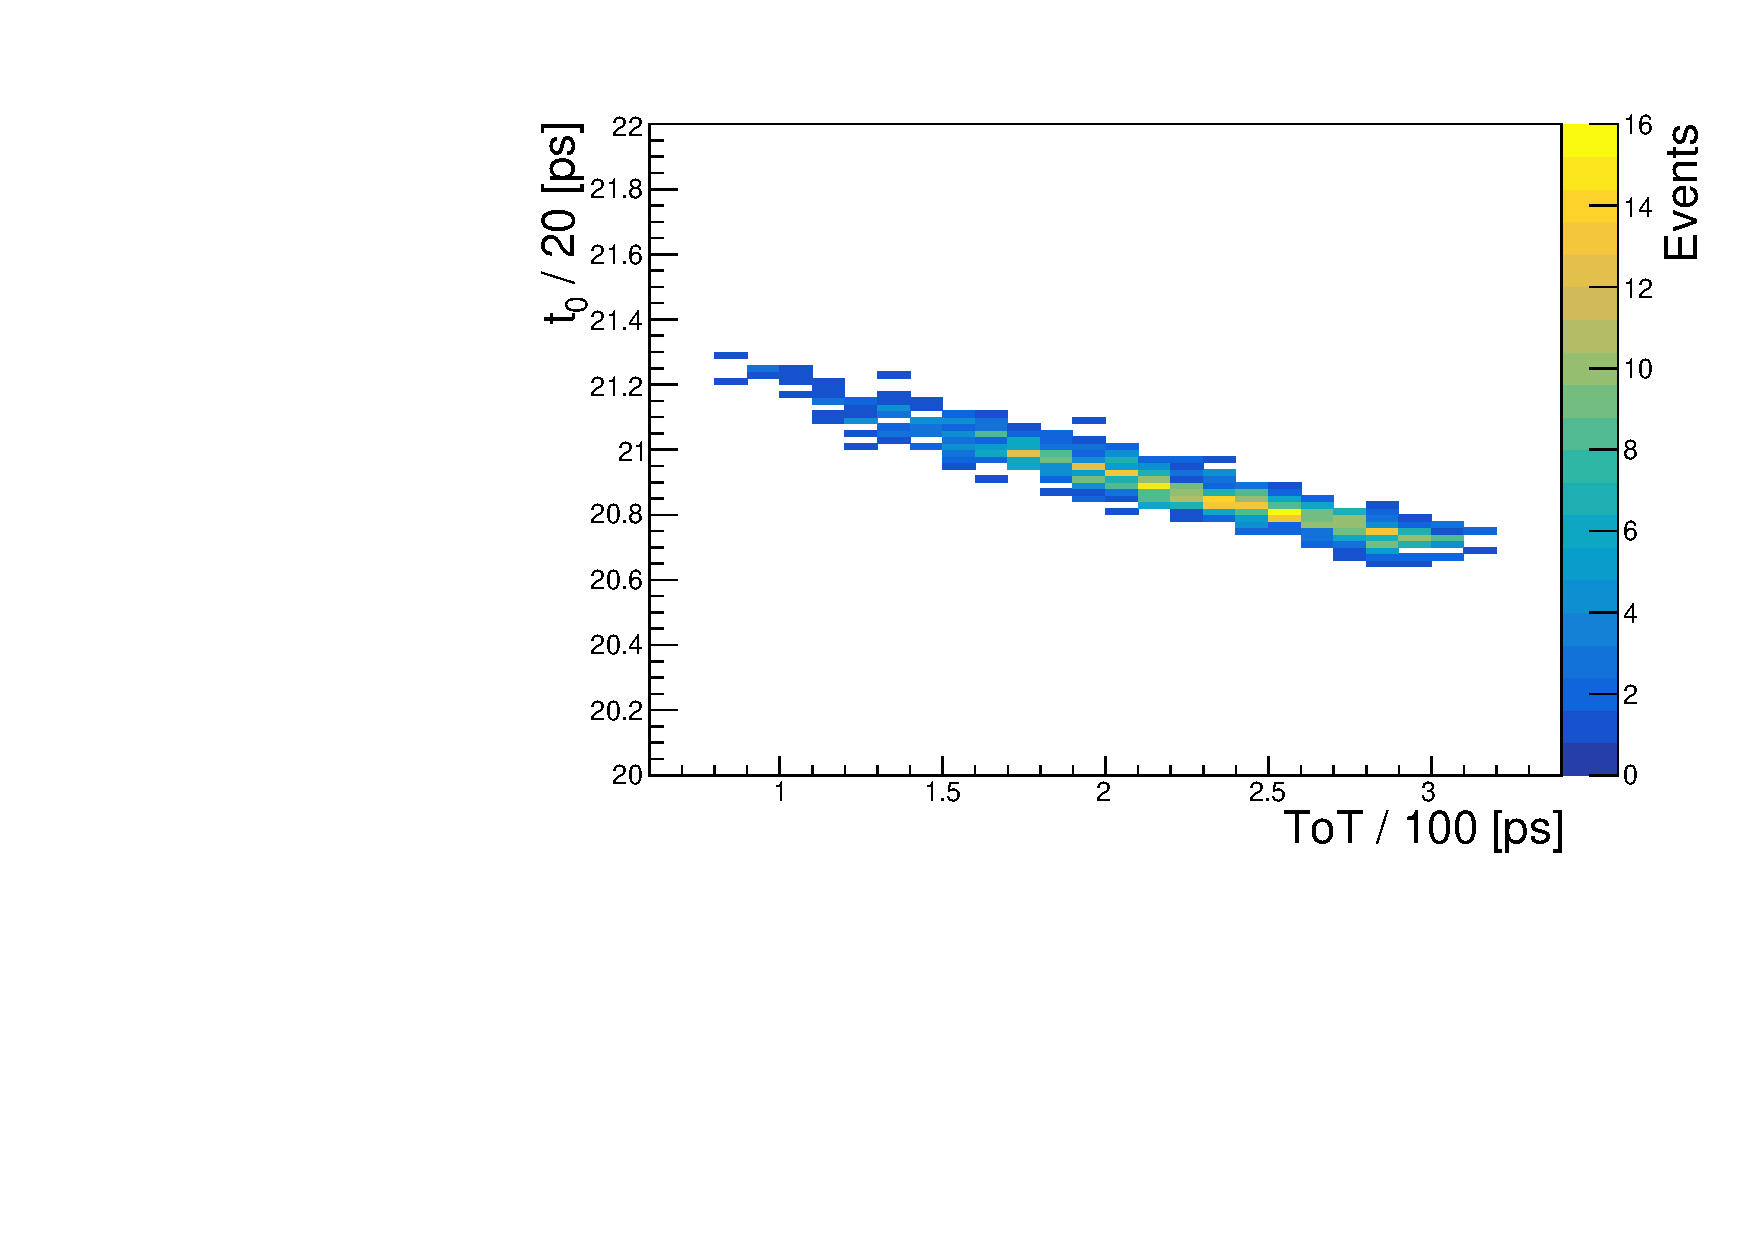
\includegraphics[width=0.48\textwidth]{figs/twoD_ToT_pre_rad_st_1ns_snr_30_le_tot_threshold_30mV_v2.pdf} \hfill
  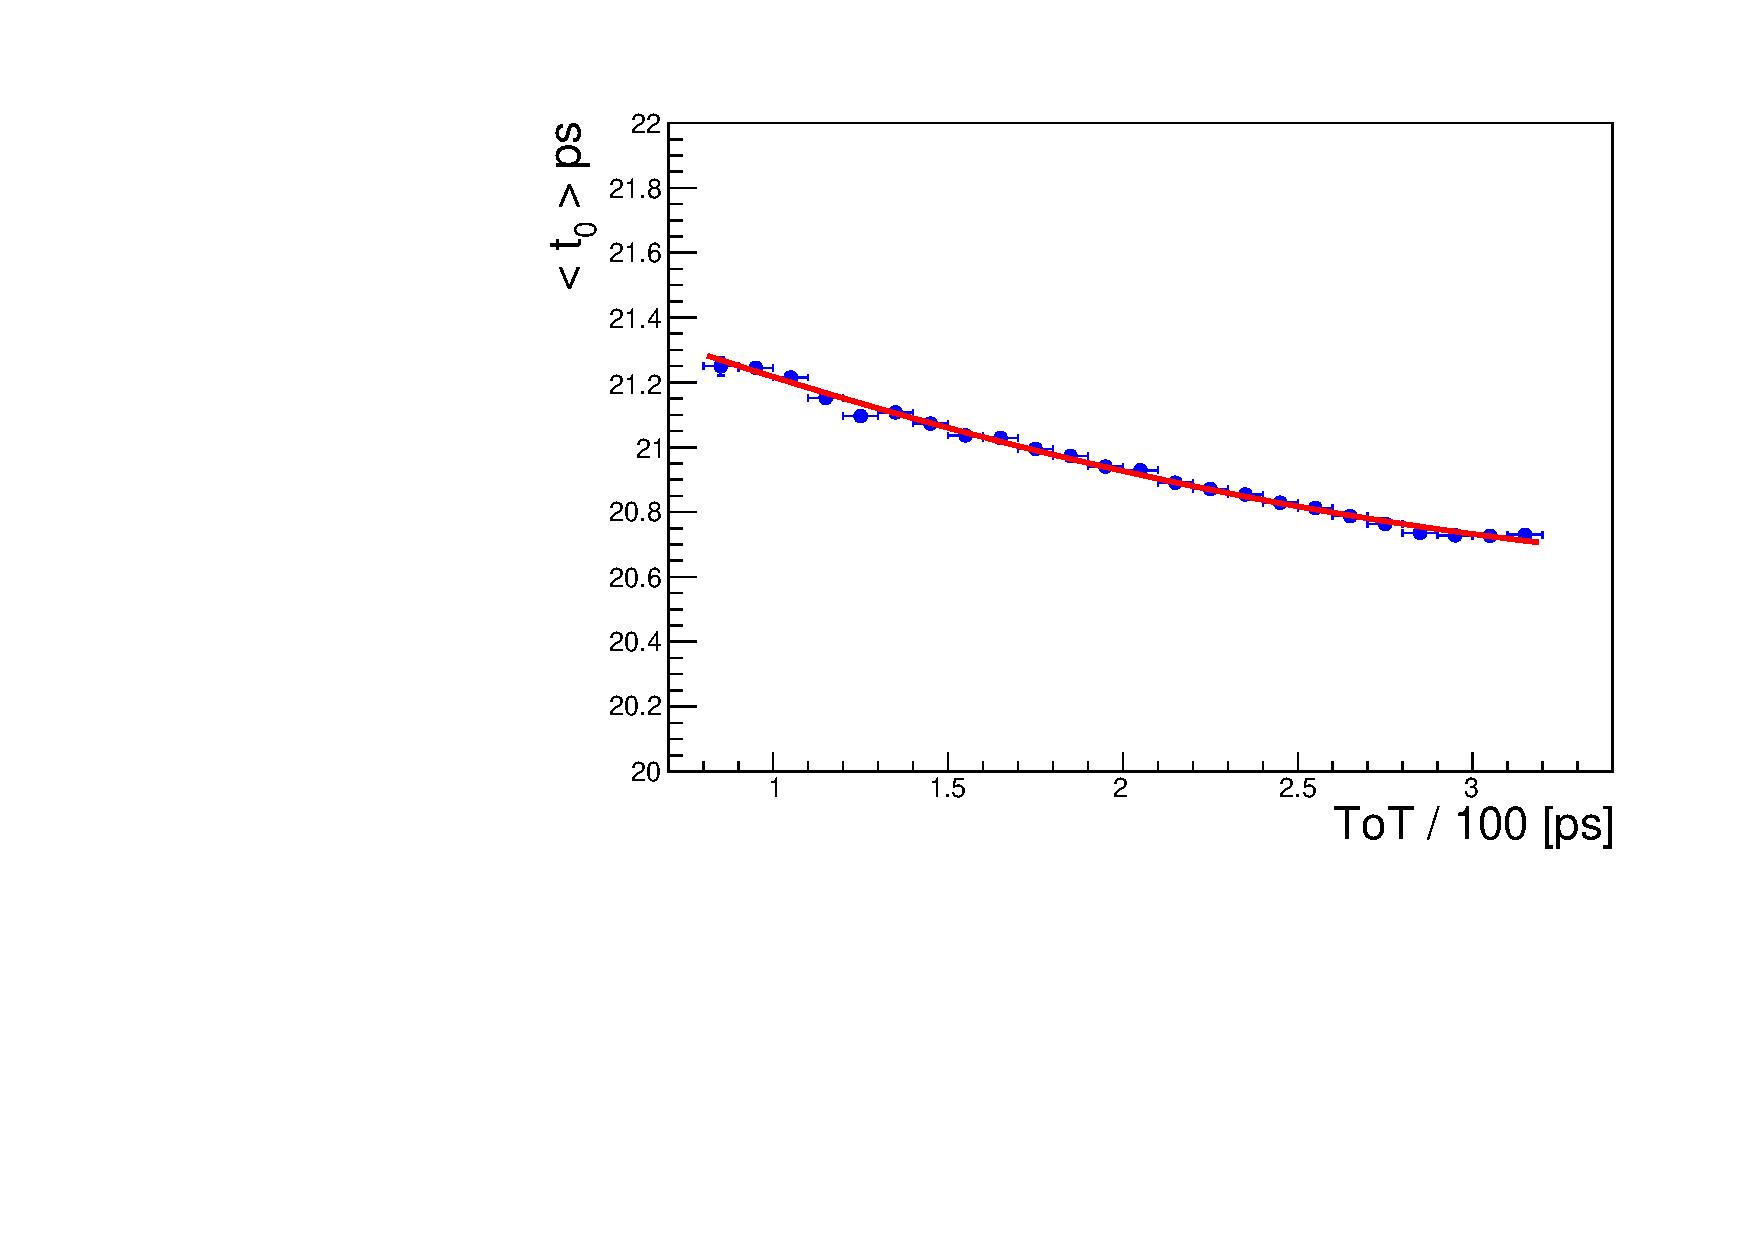
\includegraphics[width=0.48\textwidth]{figs/oneD_ToT_pre_rad_st_1ns_snr_30_le_tot_threshold_30mV_v2.pdf}
  \caption{(Left) two dimenasional map of the timestamp ($t_{0}$) and ToT ($t_{1} - t_{0}$).
  (Right) one dimensional projection of the timestamp ($t_{0}$) dependence on ToT, the red curve is the 2nd-order polinomial fit that
  ultimately is used to correct $t_{0}$. Both figures use a shaping time (ST) of 1~\si{ns} and correspond to a SNR of 30.}
  \label{fig:ToT}
\end{figure}




\section{LGAD Front-end Electronics Performance}\label{sec:results}

Herein we present a number of studies for a 50~$\mu$m LGAD. We study the time resolution as a function of irradiation
for three different scenarios: pre-radiation, and after neutron fluences of
 $5\times 10^{14}$~n/cm$^2$ and $1\times 10^{15}$~n/cm$^2$. We also quantify the effect of the BW of the FEE by varying the
 the ST ($\tau_{s}$), four STs are considerd: 0.5, 1, 2, and 4~\si{ns}. Additionally, we study the effect of noise by varying
 the SNR in all the scenarios described above. We consider three SNRs: 20, 30, and 100.
 Sec.~\ref{sec:shaping_time} summarizes the effects of the shaping time and SNR, and
and Sec.~\ref{sec:rad_tolerance} summarizes the effect of irradiation.



\subsection{Front-end electronics shaping time and SNR studies}\label{sec:shaping_time}
We scan the ST of the FEE and the SNR. The results for the pre-irradiated LGAD sensor are summarized in Table.~\ref{tab:shaping_time_prerad},
where the CF results are from the \textit{ideal} implementation. The {\color{red} split-and-delay}
 and the \textit{ideal} CFD implementations are compatible within uncertainties thus we only use one table for those results.
 We observe that the best results are consistently obtained by the 0.5~\si{ns} and 1.0~\si{ns} STs regardless of the SNR. We observe that
 longer STs are more affected by less favorable SNR. For example, for an SNR of 20, the time resolution is ~37~\si{ps} and ~100~\si{ps} for a
ST of 0.5~\si{ns} and 4.0~\si{ns}, respectively. We note that CF consistently outperforms LE, and this effect is also observed
 for less favorable SNR and slower ST. Comparing CF and LE for the 1.0~\si{ns} ST with SNR of 20 yields a difference in performance of
 26~\si{ps} (when subtrated in quadrature). Additionally, we observe that time resolutions better than 25~\si{ps} could not be achieved which
 is consistent with the known intrinsic jitter of the LGAD sensor. The latter is taken into account by the WF2 simulation and
confirmed in our study. For a SNR of 1000, essentially with zero noise, we obtained a time resolution consistent with 25~\si{ps}.
Finally, in the case of the pre-irradiated sensor we observed that time resolutions of ~35~\si{ps} are achievable for
STs between 0.5 - 1.0~\si{ns} and a SNR of 30.

The {\color{red} second order RC} CFD implementation shows a degradation on the time resolution when compared
to the {\color{red} split-and-delay}. Table.~\ref{tab:pcfd} shows the time resolution for the three SNR scenarios
studied for a 2~\si{ns} ST. We observe a 50~\si{ps} degradation for a SNR of 20 and  xx~\si{ps} degradation for a SNR of 100.

\begin{table}\label{tab:shaping_time_prerad}
    \begin{tabular}{c|ccc|ccc}
    \multicolumn{1}{c}{}& \multicolumn{6}{c}{Time Resolution (ps)} \\
    \multicolumn{1}{c}{}&\multicolumn{3}{c}{Leading Edge} & \multicolumn{3}{c}{Constant Franction}\\ \hline
    ST (ns) & SNR = 20   & SNR = 30      & SNR = 100     & SNR = 20      & SNR = 30      & SNR = 100 \\
    0.5 & $38.4 \pm 2.1$  & $34.9 \pm 1.7$  & $28.8 \pm 1.0$  & $37.2 \pm 1.9$  & $34.5 \pm 1.6$  & $29.8 \pm 1.9$ \\
    1.0 & $45.4 \pm 2.2$  & $37.3 \pm 1.4$  & $28.7 \pm 1.7$  & $36.4 \pm 1.8$  & $33.0 \pm 1.4$  & $25.9 \pm 1.3$ \\
    2.0 & $63.4 \pm 2.5$  & $47.6 \pm 2.0$  & $30.7 \pm 1.2$  & $47.6 \pm 1.9$  & $34.3 \pm 1.6$  & $28.7 \pm 1.7$ \\
    4.0 & $103.0 \pm 4.1$  & $75.3 \pm 2.8$  & $37.6 \pm 2.0$  & $73.8 \pm 3.1$  & $54.8 \pm 2.1$  & $32.1 \pm 1.3$ \\
    \end{tabular}
    \caption{50~$\mu$m pre-radiation LGAD sensor simulation: summary of best time resolution obtained for SNRs
    of 20, 30, and 100. Leading edge and constant fraction results are shown.}
 \end{table}


 \begin{table}\label{tab:pcfd}
   \begin{center}
     \begin{tabular}{c|ccc}
     \multicolumn{1}{c}{}& \multicolumn{3}{c}{Time Resolution (ps)} \\
     \multicolumn{1}{c}{}& \multicolumn{3}{c}{$\mathrm{(RC)}^{2}$ Constant Fraction}\\ \hline
     ST (ns) & SNR = 20      & SNR = 30      & SNR = 100 \\
     2.0 & $46.0 \pm xx$  & $xx \pm xx$  & $xx \pm xx$ \\
     \end{tabular}
     \caption{50~$\mu$m pre-radiation LGAD sensor using a second order RC implementation of a CFD.
     Summary of best time resolution obtained using a ST of 2\si{ns} for SNRs of 20, 30, and 100.}
   \end{center}
  \end{table}

 \begin{table}\label{tab:shaping_time_5e14}
     \begin{tabular}{c|ccc|ccc}
     \multicolumn{1}{c}{}& \multicolumn{6}{c}{Time Resolution (ps)} \\
     \multicolumn{1}{c}{}&\multicolumn{3}{c}{Leading Edge} & \multicolumn{3}{c}{Constant Franction}\\ \hline
     ST (ns) & SNR = 20   & SNR = 30      & SNR = 100     & SNR = 20      & SNR = 30      & SNR = 100 \\
     0.5 & $36.8 \pm 1.9$  & $32.0 \pm 1.3$  & $26.0 \pm 1.2$  & $32.5 \pm 1.4$  & $30.6 \pm 1.2$  & $25.1 \pm 1.2$ \\
     1.0 & $40.9 \pm 1.4$  & $33.8 \pm 1.1$  & $29.2 \pm 1.0$  & $33.4 \pm 1.5$  & $30.9 \pm 0.9$  & $26.1 \pm 1.3$ \\
     2.0 & $56.9 \pm 2.4$  & $45.3 \pm 2.2$  & $30.1 \pm 1.1$  & $43.7 \pm 1.6$  & $36.9 \pm 1.3$  & $24.4 \pm 1.0$ \\
     4.0 & $93.3 \pm 3.6$  & $67.9 \pm 2.5$  & $36.5 \pm 1.3$  & $70.8 \pm 2.8$  & $52.4 \pm 1.9$  & $29.9 \pm 1.9$ \\
     \end{tabular}
     \caption{50~$\mu$m LGAD sensor simulation after neutron fluence of
      $5\times 10^{14}$~n/cm$^2$: summary of best time resolution obtained for SNRs
     of 20, 30, and 100. Leading edge and constant fraction results are shown.}
  \end{table}

  \begin{table}\label{tab:shaping_time_1e_15}
      \begin{tabular}{c|ccc|ccc}
      \multicolumn{1}{c}{}& \multicolumn{6}{c}{Time Resolution (ps)} \\
      \multicolumn{1}{c}{}&\multicolumn{3}{c}{Leading Edge} & \multicolumn{3}{c}{Constant Franction}\\ \hline
      ST (ns) & SNR = 20   & SNR = 30      & SNR = 100     & SNR = 20      & SNR = 30      & SNR = 100 \\
      0.5 & $47.8 \pm 2.0$  & $37.6 \pm 2.0$  & $26.6 \pm 1.3$  & $41.9 \pm 1.9$  & $34.3 \pm 1.1$  & $24.1 \pm 1.0$ \\
      1.0 & $59.9 \pm 2.3$  & $46.8 \pm 1.8$  & $28.1 \pm 1.5$  & $46.5 \pm 1.9$  & $36.8 \pm 1.3$  & $23.1 \pm 0.9$ \\
      2.0 & $89.7 \pm 3.5$  & $68.2 \pm 2.6$  & $32.3 \pm 1.4$  & $64.7 \pm 2.8$  & $49.6 \pm 2.1$  & $27.3 \pm 0.9$ \\
      4.0 & $147.3 \pm 5.1$  & $109.0 \pm 4.3$  & $42.6 \pm 1.9$  & $118.6 \pm 4.0$  & $84.1 \pm 3.2$  & $33.8 \pm 1.1$ \\
      \end{tabular}
      \caption{50~$\mu$m LGAD sensor simulation after neutron fluence of
       $1\times 10^{15}$~n/cm$^2$: summary of best time resolution obtained for SNRs
      of 20, 30, and 100. Leading edge and constant fraction results are shown.}
   \end{table}




%\subsection{Timing Performace as a function of signal-to-noise ratio}
%\label{sec:snr}
\subsection{Timing performace as a function of irradiation}\label{sec:rad_tolerance}
We study the effect of irradiation on the time resolution of a 50~$\mu$m LGAD sensor. The impact of irradiation on the unprocessed
signal pulse shapes are accounted for by the WF2 simulation. We consider three cases: pre-irradiated, and neutron fluences of
$5\times 10^{14}$~n/cm$^2$ and $1\times 10^{15}$~n/cm$^2$. We perform the same studies as in the pre-irradiated case discussed in
Sec.~\ref{sec:shaping_time}. The results for the irradiated LGAD are presented in Tab.~\ref{tab:shaping_time_5e14} and
Tab.~\ref{tab:shaping_time_1e_15} for neutron fluences of
$5\times 10^{14}$~n/cm$^2$ and $1\times 10^{15}$~n/cm$^2$, respectively.
We observe similar trends to those of the pre-radiation sensor described in
Sec.~\ref{sec:shaping_time}. We note that when using STs between 0.5 - 1.0~\si{ns} and a SNR of 30, time resolutions of the order
of ~31~\si{ps} and ~37~\si{ps} are obtained for $5\times 10^{14}$~n/cm$^2$ and $1\times 10^{15}$~n/cm$^2$, respectively.

\section{Conclusion}\label{sec:conclusion}

We study the time resolution of a 50~$\mu$m LGAD sensor using a simulation framework that includes the
modeling of the raw unprocessed LGAD signal pulse, the front-end electronics, and the quantization.
We focus on the shaping time and sigal-to-noise ratio of the front-end electronics and its interplay
with the irradiation level of the sensor. We reproduce the known LGAD jitter of ~25~\si{ps}
for fast STs and large SNRs. We observe a clear degradation of the time resolution with SNR and slower STs. The best results are
obtained using a ST of 0.5~\si{ns} and using CF discriminator, and similar results are obtained with a ST of 1.0~\si{ns}. For a SNR of 30
and for STs betwen 0.5-1.0~\si{ns} we obtain time resoutions between ~30 - 37~\si{ps} for the 3 irradiations considered. The
reduction in gain with irradiation could bring the SNR for the most irradiated LGAD ($1\times 10^{15}$~n/cm$^2$) to 20 and thus
worsen the time resolution to ~42 - 47~\si{ps}. We note a clear gain in performace of CF over LE discriminators, particularly at
low SNR and the largest irradiation level. For an ST of 1.0~\si{ns} at SNR = 30, the performance improvement of CF over LE
is ~26\si{ps} for the pre-irradiated sensor and ~37\si{ps} for the irradiated sensor with neutron fluence of
$1\times 10^{15}$~n/cm$^2$. A performance degradiation is observed when using a {\color{red}second order RC} implementation of the CFD,
 specially at lower SNRs.
 Overall our simulation results indicate that time resolutions better than
45~\si{ps} are achievable for a 50~$\mu$m LGADs for irradiation levels up to neutron fluences of $1\times 10^{15}$~n/cm$^2$.


\section*{Acknowledgment}

%We thank the FTBF personnel and Fermilab accelerator's team for very good beam
%conditions during our test beam time. We also appreciate the technical support
%of the Fermilab SiDet department for the rapid production of wire-bonded and
%packaged LGAD assemblies. We would like to thank Alan Prosser and Ryan Rivera
%or their critical help in setting up the DAQ and trigger chain. We thank Ned
%Spencer, Max Wilder, and Forest McKinney-Martinez for their technical
%assistance, and the CNM and HPK manufacturing team. We acknowledge the help of
%V. Cindro and I. Mandic with the neutron irradiations.

A. Apresyan gratefully acknowledges support from DOE Early Career Research Program.

This document was prepared using the resources of the Fermi National Accelerator
Laboratory (Fermilab), a U.S. Department of Energy, Office of Science, HEP User
Facility. Fermilab is managed by Fermi Research Alliance, LLC (FRA), acting
under Contract No. DE-AC02-07CH11359. Part of this work was performed within the
framework of the CERN RD50 collaboration.

This work was supported by the Fermilab LDRD 2017.027; by the United States
Department of Energy grant DE-FG02-04ER41286; by the California Institute of
Technology High Energy Physics under Contract DE-SC0011925; by the European
Union's Horizon 2020 Research and Innovation funding program, under Grant
Agreement no. 654168 (AIDA-2020) and Grant Agreement no. 669529 (ERC
UFSD669529); by the Italian Ministero degli Affari Esteri and INFN Gruppo V; and
by the Spanish Ministry of Economy, Industry and Competitiveness through the
Particle Physics National Program (ref. FPA2014-55295-C3-2-R and
FPA2015-69260-C3-3-R) co-financed with FEDER funds.


% The Appendices part is started with the command \appendix;
% appendix sections are then done as normal sections

%\appendix
%\section{Appendix A}



% \section{}
% \label{}

%% If you have bibdatabase file and want bibtex to generate the
%% bibitems, please use
%%
%%  \bibliographystyle{elsarticle-num}
%%  \bibliography{<your bibdatabase>}

%% else use the following coding to input the bibitems directly in the
%% TeX file.

\bibliography{lgad_frontend_simulation}{}
\bibliographystyle{ieeetr}

%\begin{thebibliography}{00}

%% \bibitem{label}
%% Text of bibliographic item

%\bibitem{}

%\end{thebibliography}
\end{document}
\endinput
%%
%% End of file `elsarticle-template-num.tex'.
